% doc class article- for master thesis
\documentclass[a4paper,11pt]{article}

% installing necessary packages
\usepackage[english]{babel}
\usepackage{biblatex}
\addbibresource{Bibliography.bib}
\usepackage{amssymb}
\usepackage[a4paper,top=2cm,bottom=2cm,left=3cm,right=2cm,marginparwidth=1.75cm]{geometry}
\usepackage{amsmath}
\usepackage{graphicx}
\usepackage[colorlinks=true, allcolors=blue]{hyperref}
\usepackage{bookmark}
\usepackage{tikz}
\usetikzlibrary{calc}
\usepackage{booktabs}
\usepackage{emptypage}
\usepackage{hyperref}
 \hypersetup{ 
     colorlinks=true, 
     linkcolor=black, 
     filecolor=black, 
     citecolor = black,       
     urlcolor=black, 
}

% command for inserting keyowrds after the abstract
\providecommand{\keywords}[1]
{
  \small	
  \textbf{\textit{Keywords---}} #1
}

% command for inserting border on the title page
\newcommand\HRule{\rule{\textwidth}{1pt}}

% command for starting the section on a new page
%\AddToHook{cmd/section/before}{\clearpage}

% Font and line spacing adjustments
\usepackage{times}  % Times New Roman text
\usepackage{newtxmath}  % Times New Roman math
\usepackage{setspace}
\onehalfspacing  % Adjust line spacing to 1.5


% begin the main content of the document
\begin{document}

% all the description of the very first title page
\begin{titlepage}

%for border around first page
%\begin{tikzpicture}[remember picture, overlay]
%     \draw[line width = 1pt] ($(current page.north west) + (0.7in,-1in)$) rectangle ($(current page.south east) + (-0.7in,1in)$);
%\end{tikzpicture}

\begin{center}
    \vspace*{2cm}    
    \Large
    \textbf{Analysis of the Nested Logit Model under the BLP Framework through Simulation and Empirical Applications}
        
    \vspace{3cm}
    \large
    Master Thesis Presented to the \\
    \vspace{0.2cm}
    Department of Economics at the\\
    \vspace{0.2cm}
    Rheinische Friedrich-Wilhelms-Universität Bonn
        
    \vspace{1.5cm}

    In Partial Fulfillment of the Requirements for the Degree of\\ 
    \vspace{0.2cm}
    Master of Science (M.Sc.)
    
    \vspace{2cm}
    Economics
    
    \vspace{2cm}
    \large
    Supervisors: Prof. Dr. Christoph Breunig \\
    \vspace{1cm}
    Submitted in July 2024 by:\\
    Raunak Mehrotra\\
    Matriculation Number: 3391327
\end{center}
\end{titlepage}

\vspace*{2cm}

\thispagestyle{empty}
\tableofcontents
\hypersetup{hypertexnames=false}
\newpage

% starting numbering for the main content 
\clearpage
\pagenumbering{arabic}
\setcounter{page}{1}

\begin{abstract}

Discrete choice models are essential in econometrics for analyzing decision-making where individuals choose from a set of alternatives. These models, including the Multinomial Logit (MNL) and Nested Logit (NL) models, use the Random Utility Maximization (RUM) framework to predict choices based on observable and unobservable factors. While the MNL model is popular due to its simplicity and ease of estimation, it is often limited by the Independence of Irrelevant Alternatives (IIA) property. The NL model overcomes this by allowing correlated error terms within groups of similar alternatives, providing a more realistic representation of consumer behavior. However, the application of these models is challenged by the limited availability of individual-level data, prompting reliance on more accessible market-level data. The Berry, Levinsohn, and Pakes (BLP) model addresses this by extending the RUM framework to differentiated product markets and incorporating random coefficients to account for consumer heterogeneity and price endogeneity. Despite its robustness, the BLP model's computational intensity has led to the integration of the NL model within its framework to streamline estimation while maintaining accuracy in capturing nested choice structures. This paper explores the theoretical foundations and practical applications of these discrete choice models, highlighting their advantages and limitations. Through discussing the BLP model's capabilities and the NL model's enhancements, the potential for these models to provide valuable insights into market behavior and consumer preferences is also demonstrated.

\end{abstract}\hspace{10pt}

\keywords {Discrete Choice Models, Multinomial Logit, Nested Logit, Independence of Irrelevant Alternatives, BLP Model, Market-level Data, Competition Analysis}

\clearpage
\section{Introduction}
\phantomsection\label{sec:intro}

    In the real world, there are often circumstances wherein an individual has to choose from a set of alternatives. For instance, an employee decides between the mode of transportation (car, bus, or metro) to reach the office, or a customer selecting a product from a list of brands. \\

    The decision-makers finalize their choice based on several behavioral and observable characteristics. Hence, such a model whereby the individual selects an outcome from a list of alternatives based on certain factors is known as the 'Discrete Choice Model'. \\

    To fit within the model framework, the set of alternatives, also known as, the choice set, needs to satisfy three features\cite{Train}:\\

    \begin{itemize}
        \item The choice set must be 'mutually exclusive', that is, choosing an alternative necessarily implies not selecting other alternatives. 
        \item The choice set must be 'exhaustive', that is, all the possible alternatives are included in the choice set.
        \item The choice set must be finite. \\
    \end{itemize}

    While the first and second criteria are not restrictive, the third criterion is actually restrictive and considered the defining characteristic of the discrete choice models. The conditions of 'mutually exclusive' and 'exhaustive' can be sufficed by the researcher by appropriately defining the choice set based on the research question and availability of the data. For instance, research on the choice of drinks consumers buy while shopping can ask the decision-maker to select from tea, coffee, soft drinks, and beer. Such a choice set is neither 'mutually exclusive' nor 'exhaustive'. Since the consumer can buy multiple types of drinks, the choice set violates the first feature. The second feature is violated as it's quite possible that the consumer doesn't buy any drinks at all. In such a scenario, the condition of 'mutually exclusive' can be reestablished by redefining the choice set such that all possible combinations are covered, like choosing between caffeinated drinks and non-caffeinated drinks and so on. The condition of 'exhaustive' can be met by simply adding 'no drinks' in the choice set as an alternative or excluding the decision-makers who do not buy drinks. This also establishes the importance of available data while defining the choice set, since in the absence of a detailed dataset, excluding consumers who don't buy drinks makes more meaning. \\

    The third condition of the choice set being finite is however restrictive because it distinguishes the discrete choice models from regression models. In regression models, the dependent variable is continuous and can therefore have an infinite number of possible outcomes. The discrete choice models cannot be applied in the presence of infinite alternatives. Therefore, discrete choice models are often said to examine 'which' of the dependent variable, and the regression models estimate 'how much' of the dependent variable.\\

    Econometricians often interpret the discrete choice models in terms of the underlying behavioral model, known as the Random Utility Model (RUM). Under the random utility models, it is assumed that the decision-makers are utility maximizers, that is, the individual preferences among a set of discrete alternatives can be described with a utility function and the individual selects the alternative that provides the maximum utility \cite{Horowitz1991}. The model can be mathematically outlined as a utility function, $\mathbf{U_{ij}}$  for individual $i$ and alternative $j$, where $j = 1, 2,\cdots, J$ and $i = 1, 2, \cdots, J$. Since a researcher cannot observe all the factors that affect utility, the utility function can be represented as the sum of two components: 
    
    \begin{itemize}
        \item The systematic component that consists of the observable factors. These components can be represented as $\mathbf{V_{ij} = V(x_{ij},s_{i}})$, where $\mathbf{V_{ij}}$ is the systematic component function and it is the linear combination of the observable characteristics of the alternatives $\mathbf{x_{ij}}$ and the observable characteristics of the individuals $\mathbf{s_{i}}$.
        \item The random component that accounts for the unobserved factors. This random variable accounts for all the unobserved variables that have an impact on the utility of choosing a specific alternative. It can be represented as $\mathbf{\epsilon_{ij}}$
    \end{itemize}
    
     Hence, the utility function for an individual $i$ for alternative $j$ is, 
    
    \begin{equation*}
        \qquad \mathbf{U_{ij}} = \mathbf{V_{ij}} + \mathbf{\epsilon_{ij}}    
    \end{equation*}

    Note that here onwards unless specified, the individual index $i$ has been omitted to simplify the notation. Therefore, the utility function can be rewritten as, 

    \begin{equation*}
        \qquad \mathbf{U_{j}} = \mathbf{V_{j}} + \mathbf{\epsilon_{j}}    
    \end{equation*}

    Given the utility function for an individual, the random utility model defines the individual's choice as the alternative that provides the highest utility. This implies that the individual chooses alternative $k$ if and only if $\mathbf{U_{k} > U_{j},\forall j \neq k}$, that is, 

     \begin{equation*}
        \qquad \begin{cases}
        \mathbf{U_{k} > U_{1} \implies V_{k} + \epsilon_{k} > V_{1} + \epsilon_{1}}\\
        \mathbf{U_{k} > U_{2} \implies V_{k} + \epsilon_{k} > V_{2} + \epsilon_{2}}\\
        \vdots\\
        \mathbf{U_{k} > U_{J} \implies V_{k} + \epsilon_{k} > V_{J} + \epsilon_{J}}\\
        \end{cases} 
    \end{equation*}

    This can be rewritten as,

    \begin{equation*}
        \qquad \begin{cases}
        \mathbf{U_{k} - U_{1} = (V_{k} - V_{1}) + (\epsilon_{k} -\epsilon_{1}) > 0}\\
        \mathbf{U_{k} - U_{2} = (V_{k} - V_{2}) + (\epsilon_{k} -\epsilon_{2}) > 0}\\
        \vdots\\
        \mathbf{U_{k} - U_{J} = (V_{k} - V_{J}) + (\epsilon_{k} -\epsilon_{J}) > 0}\\        
        \end{cases} 
    \end{equation*}

    Since $\epsilon_{j}$ are not observable, a researcher can rewrite the utility function in terms of the random variable \cite{Croissant}.

    \begin{equation*}
        \qquad \begin{cases}
        \mathbf{\epsilon_{1} < (V_{k} - V_{1}) + \epsilon_{k}}\\
        \mathbf{\epsilon_{2} < (V_{k} - V_{2}) + \epsilon_{k}}\\
        \vdots\\
        \mathbf{\epsilon_{J} < (V_{k} - V_{J}) + \epsilon_{k}}\\        
        \end{cases} 
    \end{equation*}

    Hence, the probability of an individual of selecting an alternative $k$ conditional on $\epsilon_{k}$ is, 

    \begin{equation*}
        \qquad \mathbf{(P_{k}|\epsilon_{k}) = F_{-k}(\epsilon_{1} < (V_{k} - V_{1}) + \epsilon_{k},\epsilon_{2} < (V_{k} - V_{2}) + \epsilon_{k},\cdots,\epsilon_{J} < (V_{k} - V_{J}) + \epsilon_{k})}
    \end{equation*}

    Where $F_{-k}$ is the multivariate distribution of $J-1$ error terms. Using the marginal density function of $\epsilon_{k}$, $f_{k}(\epsilon_{k})$, the unconditional probability of alternative $k$ that depends on only the explained variables can be described as,

     \begin{equation*}
        \qquad \mathbf{P_{k} = \int(P_{k}|\epsilon_{k})f_{k}(\epsilon_{k})d\epsilon_{k}}
    \end{equation*}

    That is,

    \begin{equation*}
        \qquad \mathbf{P_{K} = \int F_{-k}(\epsilon_{1} < (V_{k} - V_{1}) + \epsilon_{k},\epsilon_{2} < (V_{k} - V_{2}) + \epsilon_{k},\cdots,\epsilon_{J} < (V_{k} - V_{J}) + \epsilon_{k})f_{k}(\epsilon_{k})d\epsilon_{k}}
    \end{equation*}
    \newpage    
    
    The distribution of the unobserved component of the utility function is crucial in discrete choice modeling. Different types of discrete choice models are derived based on the specified density of the random variable, denoted as $\mathbf{f(\epsilon)}$. For certain specifications of $\mathbf{f(\epsilon)}$ and under the assumption that the unobserved component of the utility function is independently and identically distributed (iid) extreme value, the resulting integral has a closed-form solution, as exemplified by the multinomial logit model. Nested logit models, which are an extension of the multinomial logit, also yield a closed-form solution for certain specifications of $\mathbf{f(\epsilon)}$. However, unlike the multinomial logit model, the nested logit model assumes that the joint distribution of the unobserved components follows a generalized extreme value (GEV) distribution \cite{Train}.\\
    
   The multinomial logit (MNL) model is one of the most commonly used choice models due to its simple mathematical structure and ease of estimation \cite{Mcfadden1972}. The popularity of the multinomial logit can be inferred from its wide applications in econometrics and marketing. The model has been used to predict consumer choices, analyze product market shares based on aggregate data, and estimate price sensitivities in various sectors \cite{Li&Huh}. The MNL model relies on specific assumptions regarding the error component: (1) the errors follow a Gumbel distribution, (2) the errors are independently and identically distributed across alternatives, and (3) the errors are independently and identically distributed across individuals \cite{Koppelman&Bhat}. However, the popularity of multinomial logit models is diminished by the 'Independence of Irrelevant Alternatives (IIA)' property. The IIA property asserts that the relative odds of choosing between any two alternatives are unaffected by the presence or absence of other alternatives. The MNL model does not inherently satisfy the IIA property, which can lead to biased estimates. The limited applicability of the MNL model due to the IIA property underscores the need for other discrete choice models that can provide efficient estimates while addressing the limitations of the IIA property.\\

    The Nested Logit (NL) model is a prominent alternative to the Multinomial Logit (MNL) model, designed to relax the restrictions imposed by the MNL model and to account for interdependence among pairs of alternatives within the same group. The NL model partitions alternatives into groups, or nests, based on similar characteristics. The error terms of alternatives within a nest are correlated, whereas the error terms of alternatives in different nests are uncorrelated. This structure allows the NL model to capture more realistic substitution patterns compared to the MNL model. The model is a specific case of the Generalized Extreme Value (GEV) model developed by McFadden, which ensures that the model is consistent with utility maximization and generates consistent estimates. This variant is known as the Utility Maximizing Nested Logit (UMNL). An alternative formulation, known as the Non-Normalized Nested Logit (NNNL), is similar to the UMNL except that it does not conform to the principles of utility maximization. Only by imposing restrictions on the nesting parameters or by introducing dummy nests can estimation results consistent with random utility theory be reached \cite{silberhorn2008estimation}.\\

    The application of discrete choice models often faces significant challenges due to the limited availability of individual-level data. Collecting detailed consumer data is not only difficult but also often prohibitively expensive, making it impractical for many studies. As a result, researchers frequently rely on market-level data, which is more accessible and can provide valuable insights into market behavior and consumer preferences.\\

    The Berry, Levinsohn, and Pakes (BLP) model is commonly used in the analysis of differentiated product markets, allowing for the estimation of demand parameters by considering the complexities of consumer choice behavior. At its core, the BLP model operates under the framework of Random Utility Maximization (RUM). A key feature of the BLP model is the incorporation of random coefficients, which account for heterogeneity in consumer preferences that cannot be fully captured by observed characteristics alone. This aspect of the model enables it to address issues of price endogeneity and varying consumer responses to product attributes. When applied to aggregate data, the BLP model utilizes market-level information such as prices, market shares, and aggregate product attributes to infer individual-level demand patterns and elasticities. Despite the lack of individual-level data, the use of random coefficients allows the BLP model to capture a broad range of consumer behaviors and market dynamics. However, this robustness comes at the cost of computational intensity, which has led researchers to explore models like the Nested Logit within the BLP framework to streamline estimation while maintaining the ability to account for the nested nature of consumer choices.\\

    Hence, the objective of this study is to review discrete choice models and to develop a comprehensive understanding of the nested logit model within the BLP (Berry, Levinsohn, and Pakes) framework. To achieve this, Section 2 discusses the Multinomial Logit (MNL) model, followed by Section 3, which examines the significance of the Independence of Irrelevant Alternatives (IIA) property. Sections 4 and 5 provide detailed reviews of the Nested Logit (NL) model and the BLP model, respectively, with Section 5 also introducing the integration of MNL and NL models within the BLP framework. In Section 6, a simulation study is conducted to evaluate the performance of the model structure developed in the previous sections. Finally, Section 7 presents the empirical application of the methodology, demonstrating its potential to address questions regarding market efficiency.\\

\clearpage

\section{Multinomial Logit Model}
\phantomsection\label{sec:MNL}

    One of the most popular discrete choice models based on maximum liklihood estimation is the multinomial logit model. An extension of the binary logit, MNL is generally used to predict the dependent variable which is nominal and has more than two categories. Meanwhile, the independent variable in the model can be categorical as well as continuous. The model must satisfy the key assumption that the error terms are extreme-value independently and identically distributed. These three hypotheses have been discussed hereby:

    \begin{itemize}

        \item \textbf{Gumbel Distribution}\\

        Generally, the most common assumption about the distribution of the error terms in statistics is that the errors are normally distributed. However, in the multinomial logit model, a normality assumption of the error terms can lead to flawed choice analysis \cite{Koppelman&Bhat}. Koppelman and Bhat (2006) also highlight the preference for Gumbel distribution in the choice model due to its computational advantages when maximization is the objective, it closely approximates the normal distribution and generates closed-form solutions. A closed-form probabilistic choice model implies that the probability can be calculated without numerical integration or simulation methods.\\

        Hence, the Gumbel distribution has the following cumulative distribution:

        \begin{equation*}
            \qquad \mathbf{P(z<t) = F(t) = \int_{-\infty}^{t} \dfrac{1}{\theta}\exp{\left(-\dfrac{z-\mu}{\theta}\right)}\exp{\left(-\exp{\left(-\dfrac{z-\mu}{\theta}\right)}\right)}dz = \exp{\left(-\exp{\left(-\dfrac{t-\mu}{\theta}\right)}\right)}}
        \end{equation*}

         and probability density function:

         \begin{equation*}
             \qquad \mathbf{f(z) = \dfrac{1}{\theta}\exp{\left(-\dfrac{z-\mu}{\theta} \right)}\exp{\left(-\exp{\left(-\dfrac{z-\mu}{\theta}\right)}\right)}}
         \end{equation*}

         respectively. Here, $\mu$ is the location parameter and $\theta$ denotes the scale parameter which determines the variance of the distribution. Further, the first two moments of the distribution, that is, the mean and variance of the distribution are given by:

         \begin{equation*}
             \qquad \mathbf{E(z) = \mu + (0.577)\theta}
        \end{equation*}
        
        \begin{equation*}
             \qquad\mathbf{V(z) = \dfrac{\pi^{2}}{6}\theta^{2}}
         \end{equation*}

         respectively. Here, $0.577$ is known as the Euler-Mascheroni constant.\\ 
         
         With respect to the MNL model, each $\epsilon$ follows a Gumbel distribution wherein the mean of $\epsilon_{j}$'s is not identified in the presence of an intercept in the $\mathbf{V_{j}}$. Then without any loss of generality, it can be assumed that $\mathbf{\mu_{j}} = 0$ $\forall j = 1, 2, \cdots, J$ alternatives. Moreover, the overall scale of utility is not identified, only $J-1$ scale parameters may be identified. The natural choice of normalization is then to impose that of one of the $\mathbf{\theta_{j}}$ as equal to $1$ \cite{Croissant}\\.   
         
        \item \textbf{Independence of Errors} \\

        If the independence of errors holds, it implies a univariate distribution of the error term. Using the mathematical notation for the random utility models as described  above, the conditional and unconditional probability of selecting an alternative can be written as:
        
        \begin{equation*}
            \qquad \mathbf{(P_{k}|\epsilon_{k}) = \prod_{k \neq j} F_{j}(V_{k} - V_{j} + \epsilon_{k})}
        \end{equation*}

        and

        \begin{equation*}
            \qquad \mathbf{P_{k} = \int \prod_{k \neq j} F_{j}(V_{k} - V_{j} + \epsilon_{k})f_{k}(\epsilon_{k})d\epsilon_{k}}
        \end{equation*}

        respectively, where $F_{j}$ is the cumulative distribution for $\epsilon_{j}$ and $f$ is the probability density function. This means that the computation of probabilities requires a solution for one-dimensional integral only.\\

        \item \textbf{Identically Distributed Errors}\\

        Through the assumption of Gumbel distribution, we know that the location parameter is not identified for any of the error terms. Therefore, the hypothesis of identically distributed errors is essentially the case of homoscedasticity, wherein the scale parameter of Gumbel distribution is the same for all alternatives. Further, as the scale parameter for one of the alternatives has been normalized to $1$, it can be assumed that in the case of homoscedasticity without any loss of generality, $\theta_{j} = 1$ $\forall j = 1, 2,\cdots, J$. The condition and unconditional probabilities can therefore be further simplified to:  

        \begin{equation*}
            \qquad \mathbf{(P_{k}|\epsilon_{k}) = \prod_{k \neq j} F(V_{k} - V_{j} + \epsilon_{k})}
        \end{equation*}

        and

        \begin{equation*}
            \qquad \mathbf{P_{k} = \int \prod_{k \neq j} F(V_{k} - V_{j} + \epsilon_{k})f_{k}(\epsilon_{k})d\epsilon_{k}}
        \end{equation*}

        where $F$ and $f$ are the Gumbel cumulative distribution and probability density functions with the location parameter, $\mu = 0$, and the scale parameter, $\theta = 1$.
    \end{itemize}

    Based on the assumptions on the distribution of the error terms and the utility function, 
    
    \begin{equation*}
        \qquad \mathbf{U_{j}} = \mathbf{V_{j}} + \mathbf{\epsilon_{j}}    
    \end{equation*}

    Where, $j = 1,\cdots, J$ and $J \ge 2$, we derive the multinomial logit model which gives the choice probabilities for each alternative as a function of the systematic portion of the utility of all the alternatives \cite{Koppelman&Bhat}. These probabilities are commonly expressed as:

    \begin{equation*}
        \qquad \mathbf{Pr(k) = \dfrac{\exp{\left(V_{i}\right)}}{\sum_{j=1}^{J}\exp{\left(V_{j}\right)}}}
    \end{equation*}

    Where $Pr(k)$ is the probability of an individual choosing an alternative $k$ and $V_{j}$ is the systematic component of the utility of alternative $j$.

\subsection{Choice Probability}
\phantomsection\label{subsec: MNL Choice Probability}

    The choice probability can be easily derived using the assumption of the error term that it has an i.i.d Gumbel distribution \cite{Croissant}. Let an alternative $k$ be the alternative selected by the decision-maker over alternative $j$, then from the assumption of Gumbel distribution and identically distributed errors,

    \begin{equation*}
        \qquad \mathbf{P(\epsilon_{j} < V_{k} - V_{j} + \epsilon_{k}) = e^{-e^{-(V_{k} - V_{j} + \epsilon_{k})}}}
    \end{equation*}

    From the assumption of independence of errors, it can therefore be stated that the probability of choosing the alternative $k$ conditional on $\epsilon_{k}$ is the product of probabilities of all alternatives except $k$, that is,

    \begin{equation*}
        \qquad \mathbf{(P_{k}|\epsilon_{k}) = \prod_{k \neq j}e^{-e^{-(V_{k} - V_{j} + \epsilon_{k})}}}
    \end{equation*}

    This implies the unconditional probability is,

    \begin{equation*}
        \qquad \mathbf{P_{k} = \int_{-\infty}^{+\infty} \left(\prod_{k \neq j}e^{-e^{-(V_{k} - V_{j} + \epsilon_{k})}}\right)e^{-\epsilon_{k}}e^{-e^{-\epsilon_{k}}}d\epsilon_{k}}
    \end{equation*}

    Expanding the above equation for all alternatives including $k$, we get,

    \begin{equation*}
        \qquad \mathbf{P_{k} = \int_{-\infty}^{+\infty} \left(\prod_{j}e^{-e^{-(V_{k} - V_{j} + \epsilon_{k})}}\right)e^{-\epsilon_{k}}d\epsilon_{k}}
    \end{equation*}

    \begin{equation*}
        \qquad \mathbf{P_{k} = \int_{-\infty}^{+\infty} \left(e^{-\sum_{j=1}^{J}e^{-\left(V_{k} - V_{j} + \epsilon_{k}\right)}}\right)e^{-\epsilon_{k}}d\epsilon_{k} = \int_{-\infty}^{+\infty} \left(e^{-e^{-\epsilon_{k}}\sum_{j=1}^{J}e^{-\left(V_{k} - V_{j}\right)}}\right)e^{-\epsilon_{k}}d\epsilon_{k}}
    \end{equation*}

    Now let, $\mathbf{y = e^{-\epsilon_{K}} \implies dy = -e^{-\epsilon_{K}}d\epsilon_{k}}$. Substituting the variable $y$ in the above equation,

    \begin{equation*}
        \qquad \mathbf{P_{k} = \int_{0}^{+\infty} \left(e^{-y}\sum_{j=1}^{J}e^{-\left(V_{k} - V_{j}\right)}\right)dy}
    \end{equation*}

    This integral has a closed-form solution,

    \begin{equation*}
        \qquad \mathbf{P_{k} = \left[-\dfrac{e^{-t\sum_{j=1}^{J}e^{-\left(V_{k}-V_{j}\right)}}}{\sum_{j=1}^{J}e^{-\left(V_{k}-V_{j}\right)}}\right]_{0}^{+\infty} = \dfrac{1}{\sum_{j=1}^{J}e^{-\left(V_{k}-V_{j}\right)}}}
    \end{equation*}

    and can be rewritten using the logit probability as,

    \begin{equation*}
        \qquad \mathbf{P_{k} = \dfrac{e^{V_{k}}}{\sum_{j=1}^{J}e^{V_{j}}}}
    \end{equation*}

\subsection{Interpretation: Marginal Effects and Elasticities}
\phantomsection\label{subsec:Interpretation}

\subsubsection{Marginal Effects}
\phantomsection\label{subsubsec:Marginal Effects}

    Unlike the linear models where coefficients can be directly interpreted as the marginal effects of the independent variable on the dependent variable, the interpretation of the coefficient in the multinomial logit models is not easy. Marginal effects are one of the techniques to quantify the change in probabilities with respect to the change in the values of the characteristics that define the utility.\\

     The explanatory variables can be classified as individual-specific ($s_{i}$) and alternative-specific ($x_{ij}$). Therefore, a researcher might be interested in knowing the change in the probability of choosing an alternative in response to a change in individual-specific characteristics or an alternative-specific characteristic. Both of these marginal effects have been covered hereby.\\

    \textbf{Alternative Specific}: Consider $P_{ik}$ be the probability for an individual $i$ selecting alternative $k$ and let $x_{ik}$ be the alternative-specific explanatory variable. Then the marginal effect is calculated by differentiating $P_{ik}$ with respect to $x_{ik}$. This measure is also known as the 'Direct Derivative' and is given by \cite{Train},

        \begin{equation*}
            \qquad \mathbf{\dfrac{\partial P_{ik}}{\partial x_{ik}} = \dfrac{\partial \left[\left(e^{V_{ik}}\right) \bigg/  \left(\sum_{j=1}^{J}e^{V_{ij}}\right)\right]}{\partial x_{ik}}}
        \end{equation*}
        \begin{equation*}
            \qquad \qquad \mathbf{ = \left[ e^{V_{ik}} \bigg/ \sum_{j=1}^{J}e^{V_{ij}} \right] \left(\dfrac{\partial V_{ik}}{\partial x_{ik}}\right) - \left[ e^{V_{ik}} \bigg/ \left( \sum_{j=1}^{J}e^{V_{ij}} \right)^{2}\right]\left(e^{V_{ik}}\right) \left(\dfrac{\partial V_{ik}}{\partial x_{ik}}\right)}
        \end{equation*}
        \begin{equation*}
            \qquad \qquad \mathbf{ = \left(\dfrac{\partial V_{ik}}{\partial x_{ik}}\right) \left( P_{ik} - P_{ik}^{2} \right)}
        \end{equation*}
        %\begin{equation*}
        %    \qquad \mathbf{\dfrac{\partial P_{ik}}{\partial x_{ik}} = \left[\dfrac{\partial V_{ik}}{\partial x_{ik}} \right](P_{ik})(1 - P_{ik})}
        %\end{equation*}

        Let $V_{ik} = \beta_{k}x_{ik}$, the observed component of the linear utility function. Then, the direct derivative can be written as

        \begin{equation*}
            \qquad \mathbf{\dfrac{\partial P_{ik}}{\partial x_{ik}} = \beta_{k}(P_{ik})(1 - P_{ik})}
        \end{equation*}

        The value of the derivative is the largest when $P_{ik} = 1 - P_{ik}$, that is, $P_{ik} = 0.5$ and becomes smaller as $P_{i}$ approaches zero or one. This implies that the impact of a change in the observed variable is the highest when the choice probability has a high degree of uncertainty and as the probability of choosing an alternative improves (that is, moves closer to zero or one), the effect of the observed variable diminishes. It can also be explicitly stated that the sign of the marginal effect is the same as the sign of the coefficient $\beta_{k}$. Hence, for an increase in $x_{ik}$, the $P_{ik}$ increase if $\beta_{k}$ is positive and decreases if $\beta_{k}$ is negative.\\

        Often it is of more interest to calculate the effect of change in the observed variable of another alternative on the choice probability of the alternative of interest. This is known as the 'Cross Derivative' and is calculated as,

        \begin{equation*}
            \qquad \mathbf{\dfrac{\partial P_{im}}{\partial x_{ik}} = \dfrac{\partial \left[\left(e^{V_{im}}\right) \bigg/ \left(\sum_{j=1}^{J}e^{V_{ij}}\right)\right]}{\partial x_{ik}}}
        \end{equation*}

        Here, $P_{im}$ denotes the choice probability of choosing alternative $m$ by an individual $i$ and $x_{ik}$ is the observed characteristic of alternative $k$. Solving the differentiation,

        \begin{equation*}
            \qquad \qquad \mathbf{ = - \left[\dfrac{\left(e^{V_{im}}\right)} {\left(\sum_{j=1}^{J}e^{V_{ij}}\right)^2}\right] e^{V_{ik}} \dfrac{\partial V_{ik}}{\partial x_{ik}}}
        \end{equation*}

        \begin{equation*}
            \qquad \qquad \mathbf{ = - \dfrac{\partial V_{ik}}{\partial x_{ik}} P_{im} P_{ik}}
        \end{equation*}

        Assuming the same linear utility representation as for the direct-derivative, $\dfrac{\partial V_{ik}}{\partial x_{ik}} = \beta_{k}$ and substituting the value in the marginal effect we get,

        \begin{equation*}
            \qquad \mathbf{\dfrac{\partial P_{im}}{\partial x_{ik}} = - \beta_{k} P_{im} P_{ik}}
        \end{equation*}

        Where, $P_{ik}$ is the choice probability of alternative $k$.\\
        
        The above derivation tells informs that there exists an inverse relation between the choice probability of an alternative and the attribute of another alternative. If the observed variable $x_{ik}$ is desirable and hence has a positive coefficient $\beta_{k}$, then an increase in $x_{ik}$ reduces the probability of choosing alternative $m$.\\

        An important outcome from the derivation of the direct and cross derivatives is that the sum of the marginal effects over all the alternatives must be zero. That is, if there is a change in the attribute of an alternative such that its choice probability increases, then the additional probability is drawn from other alternatives and hence, their choice probability necessarily decreases. This also stems from the fact that the sum of the probabilities is always one. This can be shown as,

        \begin{equation*}
            \qquad \mathbf{\sum_{k=1}^{J}}\dfrac{\partial P_{ik}}{\partial x_{ij}} = \dfrac{\partial P_{ij}}{\partial x_{ij}} + \sum_{k \neq j}\dfrac{\partial P_{ik}}{\partial x_{ij}}             
        \end{equation*}
        \begin{equation*}
            \qquad \qquad \qquad \mathbf{ = \beta_{j}(P_{ij})(1-P_{ij}) - \sum_{k \neq j}\beta_{j}P_{ik}P_{ij}}
        \end{equation*}
        \begin{equation*}
            \qquad \qquad \qquad \mathbf{ = \beta_{j}P_{ij}(1-P_{ij}) - \beta_{j}P_{ij} \sum_{k \neq j}P_{ik}}
        \end{equation*}
        \begin{equation*}
            \qquad \qquad \qquad \mathbf{ = \beta_{j}P_{ij}(1-P_{ij}) - \beta_{j}P_{ij}(1-P_{ij})} = 0
        \end{equation*}

    \textbf{Individual Specific}: Similar to alternative-specific attributes, individual-specific attributes, such as income, can also influence the choice probability of an alternative \cite{Koppelman&Bhat}. The impact of a change in such a variable on the choice probability of an alternative can be understood in two ways:

        \begin{enumerate}
            \item Direct Effect: The choice probability of an alternative $k$, denoted by $P_{ik}$, will change in response to a change in the individual-specific variable $s_{i}$, where $s_{i}$ specifically affects alternative $k$ for individual $i$. This effect can be quantified as the direct derivative of $P_{ik}$ with respect to $s_{i}$.

            \item Indirect Effect: The change in $s_{i}$ also influences the choice probabilities of all other alternatives. Consequently, the change in the choice probability $P_{ik}$ due to $s_{i}$ needs to be computed considering the impact of $s_{i}$ on alternatives other than $k$ for individual $i$. This effect is captured as the cross derivative of $P_{ik}$ with respect to $s_{i}$, reflecting how changes in $s_{i}$ alter the relative choice probabilities across all alternatives.
            \end{enumerate}

    The marginal effect of a change in $s_{i}$ on $P_{ik}$, specific to alternative $k$ is given by,

        \begin{equation*}
            \qquad \mathbf{\dfrac{\partial P_{ik}}{\partial s_{i}} = \beta_{k}P_{ik}\left(1-P_{ik}\right)} 
        \end{equation*}

        Meanwhile, the marginal effect of a change in $s_{i}$ on $P_{ik}$, specific to another alternative $j$ is given by,

        \begin{equation*}
            \qquad \mathbf{\dfrac{\partial P_{ik}}{\partial s_{i}} = - \beta_{j}P_{ik}P_{ij}}
        \end{equation*}

    Aggregating the above marginal effect over all alternatives other than $k$,

        \begin{equation*}
            \qquad \mathbf{\sum_{j \neq k}\dfrac{\partial P_{ik}}{\partial s_{i}} = - P_{ik} \sum_{j \neq k}\beta_{j}P_{ij}}
        \end{equation*}

    Therefore, the change in choice probability of an individual $i$ for alternative $k$ due to a change in an individual-specific attribute can be measured by summing up the marginal effects over all alternatives, 

        \begin{equation*}
            \qquad \mathbf{\dfrac{\partial P_{ik}}{\partial s_{i}} = \beta_{k}P_{ik}\left(1-P_{ik}\right) - P_{ik} \sum_{j \neq k}\beta_{j}P_{ij}}
        \end{equation*}
        \begin{equation*}
            \qquad \qquad \qquad \mathbf{ = P_{ik} \left(\beta_{k} - \beta_{k}P_{ik} - \sum_{j \neq k}\beta_{j}P_{ij}\right)}
        \end{equation*}
        \begin{equation*}
            \qquad \qquad \qquad \mathbf{ = P_{ik} \left(\beta_{k} - \left(\beta_{k}P_{ik} + \sum_{j \neq k}\beta_{j}P_{ij}\right)\right)}
        \end{equation*}
        \begin{equation*}
            \qquad \qquad \qquad \mathbf{ = P_{ik} \left(\beta_{k} - \sum_{j = 1}^{J} \beta_{j}P_{ij}\right)}
        \end{equation*}

    Hence, for an individual-specific variable, the marginal effect is given by 

        \begin{equation*}
            \qquad \mathbf{\dfrac{\partial P_{ik}}{\partial s_{i}} = P_{ik} \left(\beta_{k} - \sum_{j = 1}^{J} \beta_{j}P_{ij}\right)}
        \end{equation*}

    Where $\mathbf{\sum_{j = 1}^{J} \beta_{j}P_{ij}}$ is the weighted average of the coefficients for all the alternatives and the weights are given by the probability of choosing the alternatives.\\

    Further, the sign of the marginal effect is ambiguous. It will be positive only if the coefficient of alternative $k$ is larger than the weighted average of the coefficients of all the alternatives \cite{Croissant}.
        
\newpage
\subsubsection{Elasticities}
\phantomsection\label{subsubsec: Elasticities}    

    Elasticities are also a popular measure to interpret the choice probabilities since they are normalized for the variable units \cite{Train}. Elasticities are commonly defined as the percentage change in the outcome variable for a percentage change in the explanatory variable. In the context of the MNL model, the outcome variable is the choice probability of choosing an alternative, say $P_{ik}$ and the explanatory variable is the alternative-specific, $x_{ik}$ and individual-specific, $s_{i}$ attribute. Hereby, the elasticity for each of the marginal effects has been calculated.\\

    'Direct Elasticity' corresponds to the direct derivative derived above and it measures the proportional change in the choice probability of an $P_{ik}$ for a proportional change in the explanatory variable of that alternative, $x_{ik}$.

    \begin{equation*}
        \qquad \mathbf{\eta_{x_{ik}}^{P_{ik}} = \dfrac{\dfrac{\partial P_{ik}}{P_{ik}}}{\dfrac{\partial x_{ik}}{x_{ik}}} = \dfrac{\partial P_{ik}}{\partial x_{ik}} \times \dfrac{x_{ik}}{P_{ik}}}
    \end{equation*}

    $\dfrac{\partial P_{ik}}{\partial x_{ik}}$ is the direct derivative and hence its value can be substituted to get the 'Direct Elasticity'.

    \begin{equation*}
        \qquad \mathbf{\eta_{x_{ik}}^{P_{ik}} = \beta_{k}(P_{ik})(1 - P_{ik}) \times \dfrac{x_{ik}}{P_{ik}}}
    \end{equation*}
    \begin{equation*}
        \qquad \mathbf{\eta_{x_{ik}}^{P_{ik}} = \beta_{k}x_{ik}(1 - P_{ik})}
    \end{equation*}

    Similarly, the 'Cross-Elasticity' corresponds to the cross-derivative and can be derived as the percent change in the choice probability of an $P_{im}$ for a percent change in the attribute of another alternative $x_{ik}$.

    \begin{equation*}
        \qquad \mathbf{\eta_{x_{ik}}^{P_{im}} = \dfrac{\dfrac{\partial P_{im}}{P_{im}}}{\dfrac{\partial x_{ik}}{x_{ik}}} = \dfrac{\partial P_{im}}{\partial x_{ik}} \times \dfrac{x_{ik}}{P_{im}} \qquad \forall k \neq m} 
    \end{equation*}

    Substituting the value for cross-derivative to obtain the 'Cross-Elasticity'.

    \begin{equation*}
        \qquad \mathbf{\eta_{x_{ik}}^{P_{im}} = - \beta_{k}(P_{im})(P_{ik}) \times \dfrac{x_{ik}}{P_{im}}}
    \end{equation*}
    \begin{equation*}
        \qquad \mathbf{\eta_{x_{ik}}^{P_{im}} = - \beta_{k}x_{ik}P_{ik}}
    \end{equation*}

    An important property of the Multinomial Logit (MNL) model is that the cross-elasticity of choice probabilities is uniform across all alternatives in the choice set. Specifically, the cross-elasticity is independent of the particular alternative being analyzed, meaning that alternative $m$ does not appear in the formula for cross-elasticity. This property implies that if an improvement in the attribute of one alternative leads to a decrease in the choice probability of another alternative by a certain percentage, then the choice probabilities of all other alternatives, excluding the improved alternative, will also decrease by the same percentage. This uniform response to changes in attributes reflects the Independence of Irrelevant Alternatives (IIA) property inherent to the MNL model. Thus, the cross-elasticity in the MNL model serves as a restatement of the IIA property, highlighting the model's limitation in capturing nuanced changes in choice probabilities when alternatives are added or removed from the choice set.\\

    Finally, the elasticity for individual-specific attribute $s_{i}$ can also be calculated similarly.

    \begin{equation*}
        \qquad \mathbf{\eta_{s_{i}}^{P_{ik}} = \dfrac{\dfrac{\partial P_{ik}}{P_{ik}}}{\dfrac{\partial s_{i}}{s_{i}}} = \dfrac{\partial P_{ik}}{\partial s_{i}} \times \dfrac{s_{i}}{P_{ik}}} 
    \end{equation*}
    \begin{equation*}
        \qquad \mathbf{\eta_{s_{i}}^{P_{ik}} = P_{ik} \left(\beta_{k} - \sum_{j = 1}^{J} \beta_{j}P_{ij}\right) \times \dfrac{s_{i}}{P_{ik}}} 
    \end{equation*}
    \begin{equation*}
        \qquad \mathbf{\eta_{s_{i}}^{P_{ik}} = \left(\beta_{k} - \sum_{j = 1}^{J} \beta_{j}P_{ij}\right) \times s_{i}} 
    \end{equation*}\\
    
    It must be highlighted that the elasticities are calculated under the assumption that the explanatory variables are continuous. In the presence of categorical or ordinal variables, the elasticities cannot be derived, since discrete variables are not differentiable. An alternative is to measure the incremental change in the choice probability of an alternative for a unit change in a discrete attribute and then use the differences to compute the arc elasticities \cite{Koppelman&Bhat}. \\
    
    The Multinomial Logit (MNL) model is a widely used discrete choice model, valued for its straightforward mathematical formulation and ease of implementation. Its key advantages include a simple closed-form expression for choice probabilities, the ability to estimate coefficients efficiently using maximum likelihood estimation, and a clear interpretation of marginal effects. The MNL model's structure allows for the modeling of choice probabilities across multiple alternatives with a consistent and intuitive approach. However, a significant limitation of the MNL model is its inherent Independence of Irrelevant Alternatives (IIA) property. The following section will delve deeper into the implications of the IIA property

\clearpage

\section{Independence of Irrelevant Alternatives}
\phantomsection\label{sec:IIA}

    The Independence of Irrelevant Alternatives (IIA) is a fundamental property underlying the Multinomial Logit (MNL) model. The IIA property asserts that for any individual, the ratio of the probabilities of choosing between any two alternatives is unaffected by the presence or attributes of any other alternatives in the choice set \cite{Croissant}. To understand the concept better, consider $P_{l}$, $P_{m}$ and $P_{n}$ as the choice probabilities of alternatives $l$, $m$ and $n$, where

    \begin{equation*}
        \qquad \mathbf{P_{l} = \dfrac{e^{V_{l}}}{\sum_{j}e^{V_{j}}} = \dfrac{e^{V_{l}}}{e^{V_{l}} + e^{V_{m}} + e^{V_{n}}}}
    \end{equation*}
    \begin{equation*}
        \qquad \mathbf{P_{m} = \dfrac{e^{V_{m}}}{\sum_{j}e^{V_{j}}} = \dfrac{e^{V_{m}}}{e^{V_{l}} + e^{V_{m}} + e^{V_{n}}}}
    \end{equation*}
    \begin{equation*}
        \qquad \mathbf{P_{n} = \dfrac{e^{V_{n}}}{\sum_{j}e^{V_{j}}} = \dfrac{e^{V_{n}}}{e^{V_{l}} + e^{V_{m}} + e^{V_{n}}}}
    \end{equation*}

    The ratio of the three choice probabilities can then be calculated as follows,

    \begin{equation*}
        \qquad \mathbf{\dfrac{P_{l}}{P_{m}} = \dfrac{\dfrac{e^{V_{l}}}{\sum_{j}e^{V_{j}}}}{\dfrac{e^{V_{m}}}{\sum_{j}e^{V_{j}}}} = \dfrac{e^{V_{l}}}{\sum_{j}e^{V_{j}}} \times \dfrac{\sum_{j}e^{V_{j}}}{e^{V_{m}}} = \dfrac{e^{V_{l}}}{e^{V_{m}}} = e^{V_{l}-V_{m}}} 
    \end{equation*}

    Hence, the ratio of the choice probabilities are,
    
    \begin{equation*}
        \qquad \mathbf{\dfrac{P_{l}}{P_{m}} = \dfrac{e^{V_{l}}}{e^{V_{m}}} = e^{V_{l}-V_{m}}} 
    \end{equation*}
    \begin{equation*}
        \qquad \mathbf{\dfrac{P_{m}}{P_{n}} = \dfrac{e^{V_{m}}}{e^{V_{n}}} = e^{V_{m}-V_{n}}} 
    \end{equation*}
    \begin{equation*}
        \qquad \mathbf{\dfrac{P_{l}}{P_{n}} = \dfrac{e^{V_{l}}}{e^{V_{n}}} = e^{V_{l}-V_{n}}} 
    \end{equation*}

    The ratios of probabilities for each pair of alternatives depend only on the explanatory variables of those alternatives and not on the characteristics of the third alternative. In other words, the relative odds of choosing between two alternatives remain constant regardless of the introduction or removal of other alternatives.\\

    There are significant implications of the IIA property on the model framework, estimation, and the use of multinomial logit models \cite{Koppelman&Bhat}. The property allows the addition and removal of alternatives without affecting the parameters of the model. This flexibility allows the researcher to apply the model in cases where different samples face a different set of alternatives. For instance, in a study for the intercity mode of travel choice, individuals in a few sample sets would not have the choice for air travel while another sample might. Moreover, the IIA property facilitates the examination of choices among a subset of alternatives without considering the entire choice set. For instance, in the same intercity travel study, if the researcher believes that the IIA property holds, they can estimate a model using only a subset of alternatives, such as car and train, while excluding other options like air travel and bus services. This approach not only aligns with specific research requirements but also contributes to time and cost efficiencies by reducing the need for data collection on alternatives that are not relevant to the study \cite{Train}.\\

    While the Independence of Irrelevant Alternatives (IIA) property simplifies the application of the Multinomial Logit (MNL) model, it may not always hold in practice. This limitation arises because other alternatives can indeed be relevant to the ratio of probabilities between a specific pair of alternatives. When the IIA property does not hold, the MNL model can produce misleading or erroneous results. This issue is vividly illustrated by the well-known 'red bus/blue bus paradox'.\\

    \newpage
    Consider a case where a consumer can choose between taking a car and a blue bus. The probability of taking a car is $P_{c} = 3/4$ and the probability of the consumer selecting the blue bus is $P_{bb} = 1/4$. That is,
    \begin{equation*}
        \qquad \mathbf{P_{c} = \dfrac{e^{V_{c}}}{e^{V_{c}} + e^{V_{bb}}} = \dfrac{3}{4} \quad \text{and} \quad P_{bb} = \dfrac{e^{V_{bb}}}{e^{V_{c}} + e^{V_{bb}}} = \dfrac{1}{4} }
    \end{equation*}
    
    Therefore, the ratio of probabilities of the two alternatives is given by,

    \begin{equation*}
        \qquad \mathbf{\dfrac{P_{c}}{P_{bb}}  = \dfrac{e^{V_{c}}}{e^{V_{bb}}} = \dfrac{3}{1}}
    \end{equation*}
    
    Now consider that a new bus service is introduced, the 'red bus'. For simplicity, it is assumed that the red bus shares the same attributes as those of the 'blue bus' like it has the same schedule and route. The only difference between the two bus services is the color. The introduction of a new alternative provides the consumer with three choices, to drive in a car, take the blue bus, or take the red bus which can lead to a change in the choice probabilities of the alternatives. The IIA property states that the ratio of probabilities is unaffected by the presence of additional alternatives. This implies the ratio of probabilities between the car and the blue bus should remain the same $3:1$. Further, as the blue bus and red bus share the same attributes, the ratio of probabilities between the blue bus and red bus should be one. That is, since $e^{V_{bb}} = e^{V_{rb}}$,

    \begin{equation*}
        \qquad \mathbf{\dfrac{P_{bb}}{P_{rb}}  = \dfrac{e^{V_{bb}}}{e^{V_{rb}}} = 1}
    \end{equation*}

    Where, $P_{rb}$ is the probability of choosing the red bus and $V_{rb}$ comprise of the attributes of the red bus.\\

    The only probabilities for which $P_{c}/P_{bb} = 3:1$ and $P_{bb}/P_{rb} = 1:1$ is when $P_{c} = 3/5$, $P_{bb} = 1/5$, and $P_{rb} = 1/5$. These are the probabilities predicted by the multinomial logit model. However, in reality, the probability of taking a car would be expected to remain the same since consumers choose between a car and a bus, and the attributes of the buses are the same. This means that the introduction of the red bus would lead to a change in the probability of taking the blue bus which would now be split between the two buses. Hence, the choice probabilities expected post-initiation of the red bus are $P_{c} = 3/4$, $P_{bb} = 1/8$ and $P_{rb} = 1/8$.\\
    
    In this example, the multinomial logit model, because of its IIA property, overestimates the probability of taking the buses and underestimates the probability of taking the car. It predicts that the introduction of the red bus shifts consumers away from the car and the blue bus towards the red bus. Whereas in reality, the introduction of the red bus leads to a change in the ratio of probabilities of the car and blue bus, $P_{c}/P_{bb}$, rather than remaining constant as required by the MNL model. Although an extreme case, the example illustrates the strong restrictions the IIA property places on the substitution patterns in the MNL model and also emphasizes the need for alternative models that can accommodate such interdependencies among choices.\\

    The IIA property further relies on the hypothesis of the independence of the error terms. If this assumption is violated, resulting in correlated error terms, the Multinomial Logit (MNL) model can produce biased estimates. This issue can arise when two alternatives are similar, but the model fails to include variables that account for this similarity in the systematic portion of the utility function \cite{Croissant}. To see that suppose that the utilities for two alternatives are

    \begin{equation*}
        \qquad \mathbf{U_{i1} = \alpha_{1} + \beta_{1} s_{i} + \gamma x_{i1} + \epsilon_{i1}}
    \end{equation*}
    \begin{equation*}
      \qquad \mathbf{U_{i2} = \alpha_{2} + \beta_{2} s_{i} + \gamma x_{i2} + \epsilon_{i2}}
    \end{equation*}

    with $\epsilon_{i1}$ and $\epsilon_{i2}$ uncorrelated. In this situation, the MNL model can be used as the independence of error terms assumption is satisfied. But if there exists a variable $\mathbf{z_{i}}$ that is unobserved in the utility function then the estimated model is,

\newpage

    \begin{equation*}
        \qquad \mathbf{U_{i1} = \alpha_{1} + \beta_{1} s_{i} + \gamma x_{i1} + \zeta_{i1}}
    \end{equation*}
    \begin{equation*}
        \qquad \mathbf{U_{i2} = \alpha_{2} + \beta_{2} s_{i} + \gamma x_{i2} + \zeta_{i2}}
    \end{equation*}
    \begin{equation*}
        \qquad \mathbf{\zeta_{i1} = \epsilon_{i1} + z_{i}}
    \end{equation*}
    \begin{equation*}
        \qquad \mathbf{\zeta_{i2} = \epsilon_{i2} + z_{i}}
    \end{equation*}

    Due to the omitted variable bias, the error terms are now correlated which is a violation of the assumption under which the MNL model is derived. \\   
    
    The undesirable characteristics of the Independence of Irrelevant Alternatives (IIA) property—such as biased estimates and flawed inferences—undermine the effectiveness of the standard Multinomial Logit (MNL) model. The assumption of independent error terms can lead to inaccuracies when alternatives are similar but not adequately accounted for in the utility function. This limitation highlights the need for alternative models that address these deficiencies. The Nested Logit (NL) model, a special case of the Generalized Extreme Value (GEV) model developed by McFadden (1972), provides a notable solution. By relaxing the IIA property, the NL model allows for correlated error terms within predefined nests of alternatives, accommodating the possibility of similar unobserved attributes among alternatives. This relaxation enables the model to better capture complex substitution patterns and interdependencies.

\clearpage

\section{Nested Logit Model}
\phantomsection\label{sec:NL}

    %The MNL model based on the assumption that the error terms follow iid type 1 extreme value distribution is renowned due to its simple model formulation, easy estimation, and interpretation of the results. However, as discussed, the IIA property limits the scope of applicability of the model. The IIA property restricts the ratio of choice probabilities for any two alternatives to be independent of the presence of other characteristics and alternatives in the choice set. A direct implication of the IIA is that the cross-elasticity is the same for all the alternatives. However, these assumptions might not always hold. In cases where all the important variables are not accounted for by including them in the observed portion of the utility function, the error terms correlated, and this omitted variable can lead to biased parameter estimates. This generates demand for a model that holds the computational advantages of the MNL model but also overcomes the limitations put forth by the IIA property and distribution assumption of the error term.\\ 

    The Generalized Extreme Value (GEV) models encompass a range of models that exhibit diverse substitution patterns among alternatives. In GEV models, the error terms for all alternatives are jointly distributed according to a generalized extreme value distribution, which generalizes the univariate extreme value distribution used in the Multinomial Logit (MNL) model. This distribution's advantage is its ability to capture correlations among alternatives, thereby accommodating more complex substitution behaviors.\\

    When the correlation among alternatives is zero, the GEV distribution simplifies to the product of independent extreme value distributions, reducing to the standard MNL model \cite{Train}. Among the GEV models, the Nested Logit (NL) model is one of the most widely employed. The NL model is favored for its relatively simpler functional form and its ability to provide richer substitution patterns compared to the MNL model.\\

    In the Nested Logit framework, the choice process is hierarchical: consumers first select a group of alternatives, termed "nests," and then choose an alternative within the selected nest. Nests are created based on shared characteristics or similarities in unobserved attributes. For instance, in a transportation mode choice scenario, nests could be categorized into "public transportation" (e.g., bus, train) and "private transportation" (e.g., car, bike). The NL model allows for correlated error terms within each nest, reflecting unobserved preferences or factors such as convenience, cost, or comfort, which are not explicitly included in the model. Conversely, the error terms across different nests remain uncorrelated. This structure enables the Nested Logit model to capture more nuanced substitution patterns and improve modeling flexibility compared to the standard MNL model.\\ 
    
    The product alternatives are categorized into nests such that the following properties hold \cite{Train}:

    \begin{itemize}
        \item For any two alternatives that are in the same nest, the ratio of probabilities is independent of the attributes or existence of other alternatives, that is, the IIA property holds within each nest. In other words, this implies that within a nest the cross-elasticity between pairs of alternatives is the same for all pairs of alternatives in the nest.
        \item For any two alternatives in different nests, the ratio of probabilities can depend on the attributes of other alternatives in the two nests, that is, the IIA property does not hold for alternatives in different nests.
    \end{itemize}

    A two-level nested logit model is the most common choice among researchers and very few analysts estimate the nested logit models with more than three levels. The researcher decides the nesting pattern based on existing theory and casual observations \cite{Ramaul&Ramaul}. A convenient method to visualize the nesting patterns is through the tree diagram. An upside-down tree diagram denotes the nests among which the alternatives have been divided and the alternatives within each nest. However, the 'decision tree' is purely for interpretation purposes and they do not necessarily imply that an individual makes choices in a certain order, that is, the derivation of the NL model makes no assumptions about the structure of the choice process \cite{borsch2012econometric}. For instance, for a two-level decision tree, the top part of the tree shows the 'upper model', the choice between the nests $Group\_0$ and $Group\_1$, and the bottom part of the tree shows the 'lower model', the choice among alternatives $Subgroup\_2$, $Subgroup\_3$ and $Subgroup\_4$ within a nest.\\

    \begin{figure}[htb]
        \centering
        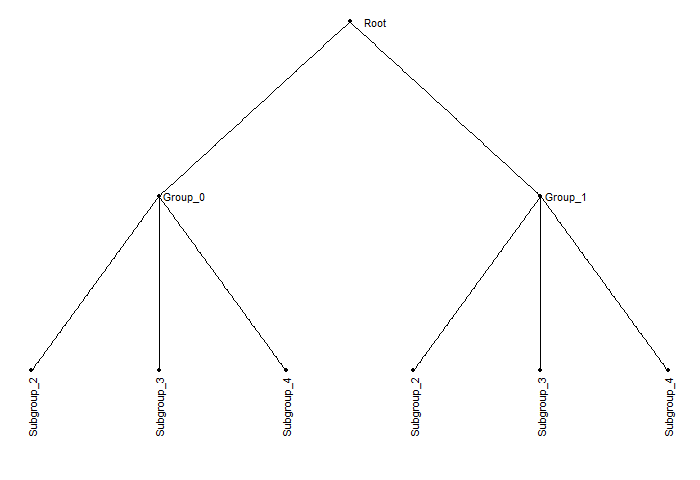
\includegraphics[width = 12cm,height = 10cm]{sim_plot.png}
        \caption{Two Level Nested Logit Model Tree Structure}
        \label{fig: Sim_Decision Tree}
    \end{figure}


\subsection{Choice Probability}
\phantomsection\label{subsec: Choice Probability}

    Consistent with the utility maximization, the following nested logit model is based on McFadden (1972). Consider a set of alternatives $j = 1, 2, \cdots J$ partitioned into $M$ subsets $B_{m}, m = 1, 2, \cdots M$ so that each alternative belongs to exactly one subset. These subsets are known as 'Nests'. As before, the utility for an individual $i$ received from an alternative $j$ can be represented as

    \begin{equation*}
        \qquad \mathbf{U_{ij} = V_{ij} + \epsilon_{ij}}
    \end{equation*}

    $V_{ij}$ represents the systematic portion of the utility observed by the researcher, and $\epsilon_{ij}$ is the random variable whose value is not observed by the researcher. The choice probability of alternative $j \in B_{m}$ for individual $i$ then can be decomposed into two parts: the probability that an alternative within the nest $B_{m}$ is chosen and the probability that the alternative $j$ is chosen given that an alternative in $B_{m}$ is chosen. Hence, the choice probability is the product of two standard logit probabilities and can be represented as,

    \begin{equation*}
        \qquad \mathbf{P_{ij} = P_{ij|B_{m}} \times P_{iB_{m}}}
    \end{equation*}

    Where, $P_{ij}$ is the probability of an individual $i$ selecting an alternative $j$ and it is the product of $P_{ij|B_{m}}$ which is the conditional probability of choosing alternative $j$ given that the nest $B_{m}$ is selected and $P_{iB_{m}}$ which is the probability of choosing some alternative in nest $B_{m}$.\\

    The error terms in the nested logit model are a generalized version of the error terms distribution in the MNL model. This special form of the GEV distribution extends the Extreme Value Type 1 distribution by allowing the alternatives within a nest to have mutually correlated error terms. The mutual correlation between error terms of alternatives within a nest is represented by an additional parameter $\tau_{m}$ in the joint distribution of error terms. Some common parameterizations of $\tau_{m}$ are $\sigma_{m} = 1 - \tau_{m}$ (McFadden (1981) \cite{McFadden}) and $\mu_{m} = 1/\tau_{m}$ (Louviere et. al. (2000) \cite{louviere2000stated}). Hereby, $\tau_{m}$ is specified to be equal to $\sqrt{1 - \rho_{m}}$ where $\rho_{m}$ is the correlation coefficient \cite{Heiss}. Since $\tau_{m}$ is an inverse measure of the correlation or an index of the dissimilarity of alternatives included in the nest $m$, it is known as the 'dissimilarity parameter', the 'nesting parameter', and the 'logsum parameter'. \\

    Based on the logsum parameter, the utilities can be rescaled by its inverse since a lower $\tau_{m}$ implies a higher correlation and vice versa. Hence, the choice probability of choosing alternative $j$  given some alternatives in its nest $B_{m}$,

    \begin{equation*}
        \qquad \mathbf{P_{j|B_{m}} = \dfrac{e^{V_{j}/\tau_{m}}} {\sum_{k \in B_{m}}e^{V_{k}/\tau_{m}}}}
    \end{equation*}

    \newpage
    The denominator of the above equation represents the measure of the attractiveness of the nest $B_{m}$. The log of the expression is known as the 'logsum variable' or the 'Inclusive Value (IV)'. It states the expected value an individual $i$ obtains from the alternatives in the nest $B_{m}$. The variable can be written as follows:

    \begin{equation*}
        \qquad \mathbf{IV_{m} = \ln \sum_{k \in B_{m}}e^{V_{k}/\tau_{m}}}
    \end{equation*}

    Finally, the probability of choosing some alternative from nest $m$ is the MNL probability for the choice between the sets. The rescaled inclusive value takes the role of the deterministic part of the utility.

    \begin{equation*}
        \qquad \mathbf{P_{B_{m}} = \dfrac{e^{\tau_{m}IV_{m}}}{\sum_{k=1}^{M}e^{\tau_{k}IV_{k}}}}
    \end{equation*}

    It is known that the RUM choice probabilities are based on the utility differences. This implies that adding a constant or scaling the utilities by a constant factor does not change the probabilities. Hence, the RUM models have to normalize the utilities. In the MNL model, the utilities are scaled such that the error terms have a variance of $\sigma^{2} = \pi^{2}/6$. Since the error terms are independent by assumption in the MNL model, their differences have a variance of $2\sigma^{2}$. However, in the NL model, the error terms are positively correlated within a nest and a higher correlation implies a lower variance of their difference. Based on the relationship between the dissimilarity parameter $\tau_{m}$ and the correlation coefficient $\rho_{m}$, the variance of the difference of the error terms is $2\sigma^{2}\tau_{m}^{2}$. The difference is further normalized by normalizing the utilities by the factor $1/\tau_{m}$ to get the variance of normalized differences as $2\sigma^{2}$. This normalization is necessary since without it the utilities in each nest would be scaled by a different factor and hence would not be comparable across nests \cite{Heiss}.\\

    The 'logsum parameter' (or the dissimilarity parameter or the nesting coefficient'), $\tau_{m}$, measures the degree of correlation between the unobserved components of alternatives in the nest $m$ and hence it also characterizes the degree of substitutability between those alternatives. To ensure consistency with the random utility maximization principles, the nesting parameter is bounded between zero and one. The interpretation of the different values of the parameter is as follows \cite{Koppelman&Bhat}:

    \begin{itemize}
        \item $\tau_{m} > 1$, this is not consistent with the theoretical derivation, Hence, the NL model is rejected.
        \item $\tau_{m} = 1$, this implies that there is zero correlation between the alternatives in the nest and so the NL model collapses to the MNL model. That is, in this case $\sum_{m=1}^{M}e^{IV_{m}} = \sum_{k=1}^{J}e^{V_{k}}$ must hold.
        \item $0 < \tau_{m} < 1$, implies a non-zero correlation among pairs of alternatives in a nest. This range of values is considered appropriate for the nested logit model. A lower value of $\tau_{m}$ indicates increased substitution among alternatives in a nest.
        \item $\tau_{m} = 0$, this case implies a perfect correlation among the pairs of alternatives in a nest. That is, the choice between the nested alternatives, conditional on the nest is deterministic.
        \item $\tau_{m} < 0$, is as well not consistent with the theoretical derivation and hence, the NL model can be rejected.
    \end{itemize}

\subsection{Estimation}
\phantomsection\label{subsec: Estimation}

    The parameters of the nested logit model can be estimated in two ways: simultaneously and sequentially \cite{Train}. Simultaneous estimation implies that the parameters are estimated using the standard maximum likelihood techniques. The choice probabilities are substituted in the log-likelihood function to obtain an explicit function of the parameters of the model. The values of the parameters that maximize this function under general conditions are consistent and efficient. The maximization of the function is sometimes difficult since the log-likelihood function is not globally concave and even in concave areas is not close to a quadratic.\\

    An alternative means to estimate the parameters of the NL model is to exploit the fact that the choice probabilities can be decomposed into marginal and conditional probabilities that are logit. Such a sequential estimation is conducted bottom-up, that is, the lower models (for the choice of alternatives within a nest) are estimated first. Then the inclusive values are calculated for each lower model using the estimated coefficients. Finally, the upper model (for choice of the nest) is estimated using inclusive values as the explanatory variable. However, there are two drawbacks of sequential estimation. First, while consistent, the standard errors of parameters of the upper model are biased downwards because the variance of the inclusive value terms is not included in the calculation of standard errors. This leads to smaller confidence intervals and larger t-statistics for the parameter estimates than true and the upper model will appear better than it is. The second drawback is that because several parameters appear in several sub-models, estimating the various upper and lower models separately provides separate estimations of the common parameters. In simultaneous estimation using maximum likelihood, the common parameters are constrained to be the same wherever they appear in the model. \\

    Therefore, these two complications imply that the sequential estimates of the nested logit mode, while consistent, are not as efficient as simultaneous estimation. A researcher should use sequential estimation if problems arise in simultaneous estimation. The estimates of the sequential estimation can be used as starting values in the simultaneous estimation. The advantage of the decomposition of the choice probability is hence, not in the estimation but in understanding the structure of the NL model.

\subsection{Elasticities}
\phantomsection\label{subsection:Elasticities}

    Similar to the Multinomial Logit (MNL) model, elasticities are crucial for interpreting choice probabilities in the Nested Logit (NL) model. As in the MNL model, direct elasticity measures the effect of a change in the attribute of an alternative on the choice probability of that alternative, while cross elasticity measures the change in the choice probability of one alternative due to a change in the attribute of another alternative. In the NL model, these elasticities are further distinguished based on whether the alternatives are in the same nest or different nests. The elasticity expressions for the NL model, along with those for the MNL model, are presented in Table 1 \cite{KoppelmanandWen}.\\

    Firstly, the direct elasticities for alternatives not within any nest are structurally identical to the MNL direct elasticities. For alternatives within a nest, the direct elasticities are greater than those for alternatives not in a nest. This reflects the intuitive notion that alternatives within a nest face more competitive pressures from similar alternatives compared to those outside any nest.\\

    Cross elasticities between pairs of alternatives depend on whether the pairs are within the same nest or in different nests. When alternatives are in different nests, the cross elasticity is structurally identical to that in the MNL model. However, when alternatives are within the same nest, the cross elasticity is larger than that for alternatives in different nests. This consistency aligns with the higher substitutability between alternatives within the same nest.\\

    The dissimilarity parameter, $\tau_{m}$, plays a crucial role in differentiating elasticity equations for nested alternatives. When, $\tau_{m} = 1$, the maximum value, the direct and cross elasticities for nested alternatives converge to the corresponding elasticities for non-nested alternatives. As $\tau_{m}$ decreases from one to zero, the direct and cross elasticities within the nest become larger than those between nests. This indicates that the sensitivity of a nested alternative to changes in its own attributes or the attributes of other alternatives within the same nest increases significantly compared to the sensitivity of non-nested alternatives.\\

    
    \begin{table}[htbp]
        \centering
        \caption{Direct and Cross-Elasticities the Nested Logit and MNL models}
        \begin{tabular}{ccc}\\
            \hline
            Model Structure & Direct-Elasticity & Cross-Elasticity\\ 
            & (change in $\mathbf{P_{j}}$ due to change in $\mathbf{x_{j}}$) & (change in $\mathbf{P_{j^{\prime}}}$ due to change in $\mathbf{x_{j}}$)\\
            \hline\\
            MNL Model & $\mathbf{(1 - P_{j}) \beta_{j} x_{j}}$ & $\mathbf{-P_{j} \beta_{j} x_{j}}$\\\\
            NL Model& $j$ not in nest & $j$ and $j^{\prime}$ not in the same nest\\
            & $\mathbf{(1 - P_{j}) \beta_{j} x_{j}}$ & $\mathbf{-P_{j} \beta_{j} x_{j}}$\\\\
            & $j$ in nest $m$ & $j$ and $j^{\prime}$ in nest $m$ \\
            & $\mathbf{\left[\left(1 - P_{j}\right) + \left(\dfrac{1}{\tau_{m}} - 1 \right)\left(1 - P_{j|m}\right)\right]\beta_{j}x_{j}}$ & $\mathbf{- \left[P_{j} + \left(\dfrac{1}{\tau_{m}} - 1\right) P_{j|m}\right] \beta_{j} x_{j}}$\\\\
            \hline
        \end{tabular}
        \label{tab:Elasticities}
    \end{table}

    The Nested Logit (NL) model not only aligns with utility maximization principles but also accounts for substitutability between alternatives. By nesting similar alternatives, the NL model relaxes the Independence of Irrelevant Alternatives (IIA) property inherent in the MNL model, leading to more realistic and interpretable estimates. This enhanced flexibility and accuracy make the NL model particularly valuable in market research and competition analysis, where understanding complex substitution patterns is crucial. Consequently, the NL model is widely adopted for its ability to provide robust, easily estimable insights into consumer choice behavior.

\clearpage

\section{BLP: Berry, Levinsohn and Pakes Model}
\phantomsection\label{sec:BLP}

    Estimation of demand has been of focus in recent studies. One of the reasons being the essential role demand plays in examining questions regarding competition, market power, and mergers.\\

    One common method for estimating demand for a set of closely related but not identical products is to specify a system of demand equations, one for each product, using market-level data. Each equation estimates the demand for a product as a function of its own price, the prices of other products, and additional variables \cite{Nevo}. However, there are several fundamental challenges in demand estimation that must be addressed \cite{BerryandHaile}.\\

    The first challenge is the endogeneity of prices, which refers to the statistical dependence between prices and unobserved factors that also affect demand. Price endogeneity can result in biased and inconsistent parameter estimates, complicating the inference of causal relationships. This issue can arise due to reverse causality or omitted variable bias. A common technique to address price endogeneity is the use of instrumental variables (IV). Instrumental variables are correlated with the endogenous variable (price) but uncorrelated with the error term. By identifying and employing appropriate instruments, it is possible to isolate the exogenous variation in prices and obtain consistent estimates. However, the challenge to demand identification extends beyond price endogeneity.\\

    Another challenge in demand estimation is that the demand for a good depends on multiple latent demand shocks. While it is straightforward to infer the impact of prices and characteristics of all related goods on the demand for a given good, the demand for a specific good also shifts in response to variations in unobserved demand shifters associated with other goods. Since prices, characteristics, and demand shocks of the focal good and all related goods cannot be excluded, they must be held constant as 'ceteris paribus' effects to measure the impact of a price change on demand. Consequently, conventional econometric techniques cannot be used to estimate demand without relying on strong functional form assumptions for identification.\\

    Aggregate data is often used for demand estimation due to the lack of availability of consumer-level data. A few commonly observed variables in market-level data are the number of goods available to consumers in each market, the prices and other characteristics of the goods, their observed market shares, and consumer characteristics. This approach to estimating discrete choice demand using market-level data was developed by Berry, Levinsohn, and Pakes (1995) \cite{blp1995}. The model can be defined as follows:

    \begin{itemize}
        \item There are $j = 1,\cdots, J$ goods available in each market/periods $t = 1, \cdots, T$. Further, $j = 0$ represents the outside good. Hence, consumer $i$ makes choice $j \in J$ in market $t$.
        \item $M$ is the market size and given by the number of consumers in that market. Then the observed market share is the quantity of good $j$ sold in market $t$ divided by the market size, that is, $s_{jt} = q_{jt}/M$ and $s_{0t} = 1 - \sum_{j=1}^{J} s_{jt}/M$.
        \item $x_{jt}$ is a vector of observable product characteristics and $p_{jt}$ is the price of product $j$ in market $t$.
        \item Finally, let $\beta$ be the vector of coefficients on the observed characteristics, $\alpha$ be the price coefficient, $\xi_{jt}$ be the product characteristics unobserved to the researcher and $\epsilon_{ijt}$ an i.i.d unobserved random shock.
    \end{itemize}

    The indirect utility function can then be written as,

    \begin{equation*}
        \qquad \mathbf{u_{ijt} = \beta_{i}x_{jt} + \alpha_{i}p_{jt} + \xi_{jt} + \epsilon_{ijt}}
    \end{equation*}

    The above equation informs three things. First, the indirect utility can be derived from a quasilinear utility function, which is free from wealth effects. Second, the unobserved product characteristics are identical for all the consumers. Since the price coefficient is allowed to vary among consumers, this assumption is consistent with the theoretical literature on vertical product differentiation. Finally, the equation assumes that all consumers face the same product characteristics. In particular, they are offered the same price. If different consumers face different prices, using an average transaction price will lead to measurement error bias. This might also lead the prices to be correlated to the error term which can be accounted for by introducing instrumental variables \cite{Nevo}.\\

    Nevo (2000) further defines individual characteristics as being composed of two components, the observed component or demographics, represented by $D_{i}$, and the unobserved component, represented by $\nu_{i}$. Since no individual data is observed, neither of the two components is directly observed. The distinction then between the components of the individual characteristics is that the researcher has a bit of knowledge on the demographics, $D_{i}$, like income, age, family size, and education, while no such information exists on additional characteristics, $\nu_{i}$, in the surveys. Formally, this can be modeled as 

    \begin{equation*}
        \qquad \mathbf{\begin{pmatrix}
            \alpha_{i}\\
            \beta_{i}
        \end{pmatrix} = \begin{pmatrix}
            \alpha\\
            \beta
        \end{pmatrix} + \Pi D_{i} + \Sigma \nu_{i}, \qquad \nu_{i} \sim P_{\nu}^{*}(\nu), D_{i} \sim \hat{P}_{D}^{*}(D)}
    \end{equation*}

    Where $P_{\nu}^{*}(\nu)$ is a parametric distribution and $\hat{P}_{D}^{*}(D)$ is a nonparametric distribution known from other data sources or a parametric distribution with parameters estimated elsewhere. The relation between the coefficients and the demographic variable, $D_{i}$, can be described as linear and affects the model's heterogeneity. By letting the parameters vary with $D_{i}$, the researcher includes more information about the distribution of the demographics in the analysis. Further, it reduces the alliance on parametric distribution.\\

    To incorporate individual characteristics in the model, let $\theta = (\theta_{1},\theta_{2})$ be a vector containing all the parameters of the model. The vector $\theta_{1} = (\alpha,\beta)$ contains the linear parameters and $\theta_{2} = (\Pi,\Sigma)$ contains the nonlinear parameters. Including these vectors in the indirect utility model,

    \begin{equation*}
        \qquad \mathbf{u_{ijt} = \delta_{jt}(x_{jt},p_{jt},\xi_{jt};\theta_{1}) + \mu_{ijt}(x_{jt},p_{jt},\nu_{i},D_{i};\theta_{2}) + \epsilon_{ijt},}
    \end{equation*}
    \begin{equation*}
        \qquad \mathbf{\delta_{jt} = x_{jt}\beta - \alpha p_{jt} + \xi_{jt}, \qquad
        \mu_{ijt} = [-p_{jt},x_{jt}](\Pi D_{i} + \Sigma \nu_{i}),}
    \end{equation*}

    Where $[-p_{jt},x_{jt}]$ is a row vector, $\delta_{jt}$ represents the mean utility and is common to all the consumers, $\mu_{ijt} + \epsilon_{ijt}$ refer to the mean-zero heteroskedastic deviation from the mean utility and it captures the effects of the random coefficients.\\

    Consumers are assumed to choose the option which offers the highest utility. Here, the consumers' utility depends on individual and product characteristics and their choice can be represented through the following choice set,

    \begin{equation*}
        \qquad \mathbf{A_{jt}(x_{.t},p_{.t},\delta_{.t};\theta_{2}) = \{ D_{i}, \nu_{i}, \epsilon_{i0t} \cdots \epsilon_{iJt} | u_{ijt} \ge u_{ilt} \qquad\forall l = 0,1,\cdots ,J\}}
    \end{equation*}

    Where $x_{.t} = (x_{lt},\cdots,x_{Jt})^{\prime}$, $p_{.t} = (p_{lt}, \cdots,p_{Jt})^{\prime}$ and $\delta_{.t} = (\delta_{lt}, \cdots, \delta_{Jt})^{\prime}$ are the observed characteristics, prices and mean utilities of all products respectively. Therefore, the choice set $A_{jt}$ defines the consumer choice for product $j$ in market $t$ over all the other products since it provides the highest utility. The error term $\epsilon_{ijt}$ is assumed to be i.i.d and distributed according to a Type-1 extreme value (Gumbel) distribution and $\nu_{i}$ is an i.i.d draw from the standard normal distribution. Further, it is also assumed that the consumer distinctly chooses a single product, that is, ties in the consumer choosing an alternative occurs with zero probability. Then the market share of the $j$th product is given by an integral over the mass of consumers in the choice set \cite{Nevo}, \cite{BerryandHaile}.\\

    \begin{equation*}
        \qquad \mathbf{s_{jt}(x_{.t},p_{.t},\delta_{.t};\theta_{2}) = \int_{A_{jt}} dP^{*}(D,\nu,\epsilon)}
    \end{equation*}
    \begin{equation*}
        \qquad \qquad \qquad \qquad \qquad \mathbf{= \int_{A_{jt}} dP^{*}(\epsilon|D,\nu), dP^{*}(\nu|D), dP_{D}^{*}(D)}
    \end{equation*}
    \begin{equation*}
        \qquad \qquad \qquad \qquad \qquad \mathbf{= \int_{A_{jt}} dP_{\epsilon}^{*}(\epsilon) dP_{\nu}^{*}(\nu) d \hat{P}_{D}^{*}(D)}
    \end{equation*}

    Where $P^{*}()$ denotes the population distribution functions.\\
    
    As the heterogeneity enters the model via $D_{i}$, $\nu_{i}$, and $\epsilon_{ijt}$, the integral defining the market share has to be computed using Monte Carlo simulation. One of the closest approximate is

    \begin{equation*}
        \qquad \mathbf{s_{jt}(x_{.t},p_{.t},\delta_{.t},P_{ns};\theta_{2}) = \dfrac{1}{ns}\sum_{i=1}^{ns}s_{ijt}}
    \end{equation*}
    \begin{equation*}
        \qquad \mathbf{= \dfrac{1}{ns}\sum_{i=1}^{ns}\dfrac{\exp\left[\delta_{jt} + \sum_{k=1}^{K} x_{jt}^{k}\left(\sigma_{k}\nu_{i}^{k} + \Pi_{k1}D_{i1} + \cdots + \Pi_{kd}D_{id}\right)\right]}
        {1 + \sum_{m = 1}{J} \exp\left[\delta_{mt} + \sum_{k=1}^{K} x_{mt}^{k}\left(\sigma_{k}\nu_{i}^{k} + \Pi_{k1}D_{i1} + \cdots + \Pi_{kd}D_{id}\right)\right]}}
    \end{equation*}

    Where $i = 1, \cdots, ns$ are random draws and $x_{jt}^{k}, \quad k = 1, \cdots, K$ are the variables that have random slope coefficients.

    
\subsection{BLP Estimator}
\phantomsection\label{subsec: Estimator}

    The random coefficients model accounts for the heterogeneity of consumer choice and endogeneity of prices due to the use of market data through nonlinear parameters $\theta_{2} = (\beta_{i},\alpha_{i})$ and instrumental variables respectively. As the identification of the model relies on instrumental variables the estimator is computed using moment conditions \cite{BerryandHaile}. Berry, Levinsohn, and Pakes (1995) proposed a generalized method of moments (GMM) estimation approach to compute the BLP estimator. The steps for BLP estimation can be sketched as follows\\

    \begin{enumerate}
        \item Calculate the market shares conditional on $\delta_{t}$ and $\theta_{2}$. This can be attained using the Monte Carlo simulation approach.
        \item For each market $t$ compute $\delta_{t}$ that equates the observed and predicted market shares, that is, $S_{t} = s_{t}(\delta_{t};\theta_{2})$. BLP proposes contraction mapping to compute the mean valuations $\delta_{t}$. That is, given a guess of $\theta_{2}$ and initial $\delta_{t}^{0}$, iterate on
        \begin{equation*}
            \qquad \mathbf{\delta_{jt}^{h+1}(\theta_{2}) = \delta_{jt}^{h}(\theta_{2}) + \log S_{jt} - \log s_{jt}(\delta_{jt}^{h};\theta_{2}),\quad j = 1,\cdots, J}
        \end{equation*}
        The iteration stops when $\mathbf{\left\|\delta_{j}^{h} - \delta_{j}^{h-1}\right\| \leq \epsilon_{in}}$. 
        \item Next step involves the computation of the GMM objective function conditional on $\delta_{t}$ and $\theta_{2}$. The GMM criterion function based on the moment condition is defined as
        \begin{equation*}
            \qquad \mathbf{\mathbb{E}\left[\xi(\theta)^{\prime} Z \right] = 0}
        \end{equation*}
        The BLP estimator is obtained by minimizing the GMM objective function
        \begin{equation*}
            \qquad \mathbf{\underset{\theta}{min} Q(\theta) = \xi(\theta)^{\prime}ZA^{-1}Z^{\prime}\xi(\theta)},
        \end{equation*}
        Where, $Z$ is a vector of appropriate instrumental variables for price, $\mathbf{A = \mathbb{E} \left[Z^{\prime} \xi(\theta) \xi(\theta)^{\prime} Z \right]}$, and \newline $\mathbf{\xi(\theta) = \delta(\theta_{2}) - (\bar{\beta}^{\prime} x_{j} - \bar{\alpha} p_{j})}$ is calculated using the estimates of $\delta$ and guessed $\theta$.
        \item As the final goal is to minimize the objective function $\mathbf{Q}$, repeat from step 1 until a minimum is found.
    \end{enumerate}

    The BLP (Berry, Levinsohn, and Pakes) random coefficients model addresses consumer heterogeneity and price endogeneity, allowing for flexible substitution patterns without the constraints imposed by prior segmentation, as seen in logit and nested logit models. However, these advantages come with certain costs. The model lacks an analytic closed-form solution, making the computation of the integral challenging. The solution for the integral in the BLP estimator is typically obtained through simulation methods and Generalized Method of Moments (GMM) estimation.\\

    Moreover, the inclusion of consumer heterogeneity necessitates additional information on the distribution of consumer heterogeneity to accurately compute market shares. This can be achieved by utilizing supplementary data sources or making parametric assumptions regarding the functional form of the distribution. These additional requirements highlight the complexity and data demands associated with the BLP model, despite its improved flexibility and accuracy in capturing consumer preferences and substitution patterns.
    
\subsection{Logit Model under the BLP Framework}
\phantomsection\label{subsec: MNL}

    The calculation of the market shares can be simplified by easing the assumptions of the BLP model such that the utility function has a closed-form analytic solution. This would imply that the consumer heterogeneity enters the model only through separable additive random shocks, $\epsilon_{ijt}$ while maintaining the distribution assumptions specified above. Therefore, we obtain an aggregate homogenous logit model wherein, $\theta_{2} = 0$, or $\beta_{i} = \beta$ and $\alpha_{i} = \alpha$. The utility function can be therefore written as

    \begin{equation*}
        \qquad \mathbf{u_{ijt} = \alpha p_{jt} + x_{jt}\beta + \xi_{jt} + \epsilon_{ijt}, \qquad \text{where,}\quad i = 1,\cdots,I, \quad j = 1,\cdots,J, \text{and}\quad t = 1,\cdots,T}
    \end{equation*}

    And the market share of brand $j$ in market $t$ is given by

    \begin{equation*}
        \qquad \mathbf{s_{jt} = \dfrac{\exp(x_{jt}\beta - \alpha p_{jt} + \xi_{jt})}
        {1 + \sum_{k=1}^{J} \exp(x_{kt}\beta - \alpha p_{kt} + \xi_{kt})} =
        \dfrac{\exp(\delta_{jt})}{1 + \sum_{k=1}^{J} \exp(\delta_{kt})}, \qquad \text{where,} \quad \delta_{jt} = x_{jt}\beta - \alpha p_{jt} + \xi_{jt}}
    \end{equation*}

    By normalizing the mean utility of the outside good, $\delta_{0t}$ to zero, its market share can be expressed as

    \begin{equation*}
        \qquad \mathbf{s_{0t} = \dfrac{1}
        {1 + \sum_{k=1}^{J} \exp(\delta_{kt})}}
    \end{equation*}

    Unlike the random coefficients model, the mean utility, $\delta_{jt}$ can be calculated by inverting the market shares. Note that, $\mathbf{\dfrac{s_{jt}}{s_{0t}} = \exp(\delta_{jt})}$. This implies that $\mathbf{\delta_{jt} = \log(s_{jt}) - \log(s_{0t})}$. Hence, 
    
    \begin{equation*}
        \qquad \mathbf{\log(s_{jt}) - \log(s_{0t}) = \delta_{jt} = x_{jt}\beta - \alpha p_{jt} + \xi_{jt}}
    \end{equation*}

    The above equation represents a regression equation for demand and can be estimated straightforwardly \cite{BerryandHaile}. To account for price endogeneity, a single market-level instrument can be included in the equation. In the absence of endogeneity, the demand equation could be estimated using Ordinary Least Squares (OLS). However, due to the potential for persistent price endogeneity, the inclusion of an instrument necessitates the use of the Two-Stage Least Squares (2SLS) method for estimation. Consequently, compared to the random coefficients model, demand estimation using the aggregate logit model is simpler and more straightforward.\\
    
    However, there are a few problems with the model. These issues can be explained using the elasticities of the logit model.

    \begin{equation*}
        \qquad \text{Own Elasticity :} \quad \mathbf{\eta_{j} = \left(\dfrac{\partial s_{j}}{\partial p_{j}}\right) \dfrac{p_{j}}{s_{j}} = \alpha p_{j}\left(1 - s_{j}\right) }
    \end{equation*}

    \begin{equation*}
        \qquad \text{Cross Elasticity :} \quad \mathbf{\eta_{jk} = \left(\dfrac{\partial s_{j}}{\partial p_{k}}\right) \dfrac{p_{k}}{s_{j}} = -\alpha p_{k}s_{k} }
    \end{equation*}

    In the own-price elasticity of demand, given that market shares are typically small, elasticity is directly proportional to the product's own price. Consequently, lower-priced brands exhibit lower elasticity, leading to higher markups, whereas high-priced goods tend to be more price elastic. This relationship, however, may not always hold true. The functional form of the price in the model underpins this relation. If the indirect utility were a function of the logarithm of price, the implied elasticity would align more consistently with theoretical expectations. Thus, the functional form significantly influences price elasticity patterns.\\

    The cross-price elasticity in the logit model indicates that the cross-elasticity of product $j$ with respect to the price of product $k$ depends solely on the price and market share of product $k$. This implies that cross-elasticity is identical across products, irrespective of differences in product characteristics. This limitation exemplifies the failure of the IIA property in the multinomial logit model. Nevo (2000) illustrates the cross-elasticity issue through the cereal data. Consider a children's cereal product 'A' and a nutrition cereal product 'B' with similar market shares, then the cross-elasticity of the logit model suggests that the substitution from another children's cereal product 'C' toward either of them will be the same. Intuitively, the substitution between product 'A' and 'C' would be expected to be higher than between 'B' and 'C'. Hence, the logit model restricts the substitution towards brands in proportion to the market shares regardless of the characteristics.\\

    

\subsection{Nested Logit Model under the BLP Framework}
\phantomsection\label{subsec: NLM}

    To incorporate the possibility of market segmentation, an aggregate nested logit model can be adopted. The two-level nested logit model is frequently used in research studies and is also employed in the subsequent sections of 'simulation study' and 'empirical application'. Therefore, the model specification discussed here is an aggregate two-level nested logit model as well. \\

    Incorporating a nested logit model within the BLP (Berry, Levinsohn, and Pakes) framework offers several advantages, notably the transformation into a linear estimating equation for a cross-section of products, which simplifies estimation as demonstrated by Berry (1994) \cite{berry1994estimating} and further extended by Björnerstedt and Verboven (2016) \cite{Björnerstedt&Verboven2016}. Björnerstedt and Verboven (2016) also address the issue of own-price elasticity within this framework.\\

    The BLP model typically employs a utility function where price enters linearly or additively with income, implying that consumers purchase only one unit of their preferred good. While this assumption is suitable for certain goods like automobiles, it may not be as appropriate for frequently purchased commodities. To address this, Björnerstedt and Verboven propose an alternative utility specification known as the constant expenditures specification. This specification differs from the unit demand approach in three key ways: (1) prices enter logarithmically rather than linearly, (2) market shares are measured in terms of value rather than volume, and (3) the potential market is defined by the potential budget instead of the potential number of consumers. Therefore, the aggregate two-level nested logit model proposed by Björnerstedt and Verboven (2016) is illustrated here.\\

    Consider the indirect utility function,

    \begin{equation*}
        \qquad \mathbf{u_{ij} = x_{j}\beta + \alpha f(y_{i},p_{j}) + \xi_{j} + \epsilon_{ij}}
    \end{equation*}

    Where, $i = 1, \cdots, I$ are the consumers, and each consumer chooses one out of $J+1$ differentiated products, $j = 0, 1, \cdots, J$. Here good $0$ represents the outside good or the no-purchase alternative. As before $x_{j}$ is the vector of observed product characteristics of product $j$, $\xi_{j}$ is a vector of product characteristics of product $j$ unobserved by the researcher and $\epsilon_{ij}$ is the random utility term. $f(y_{i},p_{j})$ represents the function through which income and price enter the model non-additively and enable consumers to purchase multiple units of the product of their choice. For simplification purposes, the time subscript $t$ has been dropped.\\

    The next step in the estimation of the aggregate demand system would involve the individual consumers' decision regarding the number of units of the preferred product they buy. The demand for the preferred good $j$ by consumer $i$ can then be calculated using Roy's identity.

    \begin{equation*}
        \qquad \mathbf{d_{ij} = - \left(\dfrac{\partial f(y_{i}, p_{j})}{\partial p_{j}} \bigg/ \dfrac{\partial f(y_{i}, p_{j})}{\partial y_{i}}\right)}
    \end{equation*}

    \newpage
    The price function $f(y_{i},p_{j})$ for two utility specifications is expressed as follows 

    \begin{equation*}
        \qquad \text{Unit Demand :} \quad \mathbf{f(y_{i},p_{j}) = y_{i} - p_{j} \implies d_{ij} = 1}
    \end{equation*}
    \begin{equation*}
        \qquad \text{Constant Expenditures :} \quad \mathbf{f(y_{i},p_{j}) = \gamma^{-1}\ln y_{i} - \ln p_{j} \implies d_{ij} = \gamma\dfrac{y_{i}}{p_{j}}}
    \end{equation*}

    The individual buys a fixed unit of good $j$ in case of unit demand and a constant fraction of her budget, $\gamma$, in case of constant expenditures specification.\\

    Given the demand decision, the next step in the process is to identify which product the consumer chooses. This can be achieved through random utility maximization. Assuming that the consumer $i$ chooses product $j$ to maximize the utility level $u_{ij}$, the utility function can be rewritten as,

    \begin{equation*}
        \qquad \mathbf{u_{ij} = K_{i} + \delta_{j} + \epsilon_{ij}}
    \end{equation*}

    where '$K_{i} = \alpha y_{i}$' in unit demand specification and '$K_{i} = \alpha\gamma^{-1}\ln y_{i}$' in constant expenditures specification. $\delta_{j}$ as before denotes the mean utility of product $j$.\\ 
    
    While in the case of outside good, the mean utility is normalized to zero, $\delta_{0} = 0$, the mean utility, $\delta_{j}$, for the other utility specifications is represented as follows

    \begin{equation*}
        \qquad \text{Unit Demand :} \quad \mathbf{\delta_{j} = x_{j}\beta + \alpha p_{j} + \xi_{j}}
    \end{equation*}
    \begin{equation*}
        \qquad \text{Constant Expenditures :} \quad \mathbf{\delta_{j} = x_{j}\beta + \alpha\ln p_{j} + \xi_{j}}
    \end{equation*}

    The model structure of the two-level nested logit model is the same as defined before. $\epsilon_{ij}$ follows the extreme type-1 value distributional assumption. The products are partitioned into $G$ groups, $g = 0, 1, \cdots, G$, where $g = 0$ only consists of the outside good. Each group is thereby further partitioned into $H_{g}$ subgroups, $h = 1, \cdots, H_{g}$. Each subgroup $h$ of group $g$ contains $J_{hg}$ products so that $\sum_{g = 1}^{G} \sum_{h = 1}^{H} J_{hg} = J$.\\ 
    
    Based on the two-level nested logit model structure and the assumption of random utility maximization, the probability that the consumer $i$ chooses product $j$ is given by

    \begin{equation*}
        \qquad \mathbf{s_{j} = s(\delta,\sigma) \equiv \dfrac{\exp((\delta_{j})/(1 - \sigma_{1}))}{\exp(\mathit{I_{hg}}/(1 - \sigma_{1}))} \dfrac{\exp(\mathit{I_{hg}}/(1 - \sigma_{2}))}{\exp(\mathit{I_{g}}/(1 - \sigma_{2}))} \dfrac{\exp(\mathit{I_{g}})}{\exp(\mathit{I})}},
    \end{equation*}

    where $\mathit{I_{hg},I_{g}}$, and $\mathit{I}$ are the 'inclusive values'. The inclusive values are expressed as,

    \begin{equation*}
        \qquad \mathbf{\mathit{I_{hg}} \equiv (1 - \sigma_{1}) \ln \sum_{k = 1}^{J_{hg}} \exp((\delta_{k})/(1 - \sigma_{1}))}
    \end{equation*}
    \begin{equation*}
        \qquad \mathbf{\mathit{I_{g}} \equiv (1 - \sigma_{2}) \ln \sum_{h = 1}^{H_{g}} \exp(\mathit{I_{hg}}/(1 - \sigma_{2}))}
    \end{equation*}
    \begin{equation*}
        \qquad \mathbf{\mathit{I} \equiv \ln \left(1 + \sum_{g = 1}^{G} \exp(\mathit{I_{g}}) \right) },
    \end{equation*}

    In the choice probability, $s(\delta,\sigma)$, $\delta$ is a $J \times 1$ vector containing the mean utilities $\delta_{j}$, and $\sigma = (\sigma_{1},\sigma_{2})$ are the nesting parameters of the nested logit model. They measure the correlation across the products of the same subgroup ($\sigma_{1}$) and group ($\sigma_{2}$).\\

    \newpage
    The aggregate demand for product $j$ can now be derived as the probability that a consumer buys product $j$, '$s_{j}$', times the quantity purchased, '$d_{ij}$', summed over all the consumers. Under the two utility specifications the aggregate demand for $j = 1, \cdots, J$ is as follows,

    \begin{equation*}
        \qquad \text{Unit Demand :} \quad \mathbf{q_{j} = \sum_{i = 1}^{I} s_{j}d_{ij} = s_{j}I}
    \end{equation*}
    \begin{equation*}
        \qquad \text{Constant Expenditures :} \quad \mathbf{q_{j} = \sum_{i = 1}^{I} s_{j}d_{ij} = s_{j}\dfrac{B}{p_{j}}}
    \end{equation*}

    where, $B = \gamma Y$ and $Y = \sum_{i=1}^{I} y_{i}$. Hence, $B$ is the total budget allocated to the products and is calculated as a fraction $\gamma$ of the total income of all the consumers.\\

    The final goal is to estimate the parameters $(\alpha,\beta,\sigma)$ that enter the aggregate demand. A linear estimable equation with $\xi_{j}$ as the error term is required to calculate the parameters, which can be derived in two steps. Firstly, following Berry (1994), the system choice probabilities are inverted to solve for the mean utilities $\delta_{j}$.\\ 
    
    The inverted choice probability system for a two-level aggregate nested logit model is given by,

    \begin{equation*}
        \qquad \mathbf{\delta_{j} = \ln(s_{j}/s_{0}) - \sigma_{1}\ln(s_{j|hg}) - \sigma_{2}\ln(s_{h|g})},
    \end{equation*}

    where $s_{j}$ is the market share of product $j$ in the market, $s_{j|hg}$ is the market share product $j$ in its subgroup $h$ of group $g$ given that an alternative is chosen and $s_{h|g}$ is the market share of subgroup $h$ in group $g$ given that group $g$ is chosen.\\

    Substituting the inverted choice probability system into the expression for the mean utilities, $\delta_{j}$ to get the estimating equations.

    \begin{equation*}
        \qquad \text{Unit Demand :} \quad \mathbf{\ln(s_{j}/s_{0}) - \sigma_{1}\ln(s_{j|hg}) - \sigma_{2}\ln(s_{h|g}) = x_{j}\beta + \alpha p_{j} + \xi_{j}}
    \end{equation*}
    \begin{equation*}
        \qquad  \qquad \mathbf{\ln(s_{j}/s_{0}) = x_{j}\beta + \alpha p_{j} + \sigma_{1}\ln(s_{j|hg}) + \sigma_{2}\ln(s_{h|g}) + \xi_{j}}
    \end{equation*}
    
    \begin{equation*}
        \qquad \text{Constant Expenditures :} \quad \mathbf{\ln(s_{j}/s_{0}) - \sigma_{1}\ln(s_{j|hg}) - \sigma_{2}\ln(s_{h|g}) = x_{j}\beta + \alpha\ln p_{j} + \xi_{j}}
    \end{equation*}
    \begin{equation*}
        \qquad  \qquad \mathbf{\ln(s_{j}/s_{0}) = x_{j}\beta + \alpha \ln p_{j} + \sigma_{1}\ln(s_{j|hg}) + \sigma_{2}\ln(s_{h|g}) + \xi_{j}}
    \end{equation*}
    
    The next step is to use the aggregate demand expressions to write the unobserved choice probabilities as observables. In the case of the unit demand specification, the choice probabilities are equal to the market shares in volume terms.

    \begin{equation*}
        \qquad \mathbf{s_{j} = \dfrac{q_{j}}{I}, \quad 
        s_{j|hg} = \dfrac{q_{j}}{\sum_{j \in H_{hg}} q_{j}}, \quad 
        s_{h|g} = \dfrac{\sum_{j \in H_{hg}} q_{j}}{\sum_{h = 1}^{H_{hg}}\sum_{j \in H_{hg}} q_{j}}, \quad 
        s_{0} = 1 - \dfrac{\sum_{j = 1}^{J} q_{j}}{I}} 
    \end{equation*}

    and in the constant expenditures specification, they are equal to the market shares in terms of value.
    
    \begin{equation*}
        \qquad \mathbf{s_{j} = \dfrac{p_{j}q_{j}}{B}, \quad 
        s_{j|hg} = \dfrac{p_{j}q_{j}}{\sum_{j \in H_{hg}} p_{j}q_{j}}, \quad 
        s_{h|g} = \dfrac{\sum_{j \in H_{hg}} p_{j}q_{j}}{\sum_{h = 1}^{H_{hg}}\sum_{j \in H_{hg}} p_{j}q_{j}}, \quad 
        s_{0} = 1 - \dfrac{\sum_{j = 1}^{J} p_{j}q_{j}}{B}} 
    \end{equation*}

    \newpage
    The estimating equation for both of the utility specifications can be estimated using instrumental variables regression of market shares on the product characteristics, prices, subgroup market shares, and group market shares. Note that based on McFadden (1972), the model is consistent with random utility maximization if $\alpha < 0$ and $1 \geq \sigma_{1} \geq \sigma_{2} \geq 0$. A negative price coefficient implies the expectation that higher prices reduce the utility and thus the probability of choosing an alternative. When $\sigma_{1}$ is high, the consumer preferences are strongly correlated among the products of the same subgroup, and when $\sigma_{2}$ is high, consumer preferences are also highly correlated across the products of the same group. If $\sigma_{1}=\sigma_{2}$, the model reduces to a one-level nested logit model wherein groups are the nests. If $\sigma_{2} = 0$, the model reduces to a one-level nested logit model with the subgroups as the nests. Finally, if $\sigma_{1} = \sigma_{2} = 0$, then the model reduces to a simple logit model without nests.\\ 

    Björnerstedt and Verboven (2016) \cite{Björnerstedt&Verboven2016} also report the formula to calculate the own-price elasticity and cross-price elasticity for a two-level nested logit model. The cross-price elasticity can be further segmented into three categories: (1) when both the products $j$ and $k$ are in the same subgroup, (2) when products $j$ and $k$ are in different subgroups of the same group, and (3) when products $j$ and $k$ are in different groups. The expression in the case of unit demand specification is,

    \begin{equation*}
        \qquad \mathbf{\dfrac{\partial q_{j}}{\partial p_{k}} \dfrac{p_{k}}{q_{j}} = \alpha \left(\dfrac{1}{1-\sigma_{1}}D_{jk}^{1} - \left( \dfrac{1}{1-\sigma_{1}} - \dfrac{1}{1-\sigma_{2}}\right)s_{j|hg}D_{jk}^2 - \dfrac{\sigma_{2}}{1-\sigma_{2}}s_{j|g}D_{h|g}^{3} - s_{j} \right)p_{j}}
    \end{equation*}
    
    Here, $s_{j|g}$ defines the market share of product $j$ in group $g$. $D_{jk}^{1} = 1$ if $j=k$ else $0$, $D_{jk}^{2} = 1$ if $j$ and $k$ are in the same subgroup otherwise $0$ and $D_{jk}^{3} = 1$ if $j$ and $k$ are in the same group and otherwise $0$.\\

    This implies that the own-price elasticity for the two-level nested logit model for the unit demand specification is given by,

    \begin{equation*}
        \qquad \mathbf{\dfrac{\partial q_{j}}{\partial p_{j}} \dfrac{p_{j}}{q_{j}} = \alpha \left(\dfrac{1}{1-\sigma_{1}} - \left( \dfrac{1}{1-\sigma_{1}} - \dfrac{1}{1-\sigma_{2}}\right)s_{j|hg} - \dfrac{\sigma_{2}}{1-\sigma_{2}}s_{j|g} - s_{j} \right)p_{j}}
    \end{equation*}

    The cross-elasticity for the case where products $j$ and $k$ are in the same subgroup can also be calculated in a similar manner,

    \begin{equation*}
        \qquad \mathbf{\dfrac{\partial q_{j}}{\partial p_{k}} \dfrac{p_{k}}{q_{j}} = \alpha \left( - \left( \dfrac{1}{1-\sigma_{1}} - \dfrac{1}{1-\sigma_{2}}\right)s_{j|hg}D_{jk}^2 - \dfrac{\sigma_{2}}{1-\sigma_{2}}s_{j|g}D_{h|g}^{3} - s_{j} \right)p_{j}}
    \end{equation*}

    Then the cross-elasticity for the case, when $j$ and $k$ are in the same groups, is,

    \begin{equation*}
        \qquad \mathbf{\dfrac{\partial q_{j}}{\partial p_{k}} \dfrac{p_{k}}{q_{j}} = \alpha \left( - \dfrac{\sigma_{2}}{1-\sigma_{2}}s_{j|g}D_{h|g}^{3} - s_{j} \right)p_{j}}
    \end{equation*}

    Finally, the cross-elasticity for the case, when $j$ and $k$ are in different groups, is 

    \begin{equation*}
        \qquad \mathbf{\dfrac{\partial q_{j}}{\partial p_{k}} \dfrac{p_{k}}{q_{j}} = \alpha \left( - s_{j} \right)p_{j}}
    \end{equation*}

    The elasticities for constant expenditures specification can also be calculated in a similar manner. The own-price elasticity in the nested logit model is still driven by the functional-form assumption, necessitating the use of theoretically sound functional forms to ensure accurate elasticity estimates. Due to the error term, $\epsilon_{ijt}$, being decomposed into an i.i.d. random shock and a group-specific component, it would be expected that the products within the same subgroup are more highly correlated than those in different subgroups and groups. This could possibly lead to a comparatively higher cross-price elasticity for pairs of alternatives within the same groups than those in different groups.
    
\newpage
\subsection{Instrumental Variables}
\phantomsection\label{subsec: IV}

    Due to the endogeneity issues in the BLP model, the parameter estimates can be biased and inconsistent. A method to address the issue is by adding exogenous instrumental variables in the model. However, there is no distinct set of variables that can be used as an instrument for all data sets belonging to different industries. Rather, the literature offers a few possible solutions that can provide exogenous variation in prices and other endogenous variables \cite{BerryandHaile}.

    \begin{itemize}
        \item Cost Shifters and Their Proxies - A standard approach to search for demand-side instrumental variables is to look for variables that shift cost and are uncorrelated with the demand shock, $\xi_{t}$. These can for instance be exogenous marginal costs, a tax, or a tariff. Proxies of a producer's actual cost shifters can also be used as an instrument. For instance, the average wage in a labor market can be a proxy for the producers' labor cost and be included as an instrument in the demand model as long as it is uncorrelated with the demand shocks conditional on the exogenous variables and consumer-specific measures (like income, education) which are also included in the model. However, the rarity of detailed data on cost shifters which vary by brand makes it challenging to use them as instruments.
        \item Hausmann Instrument - Under this, the price for the same good in another geographic market is used as an instrument for the price in the model. It assumes that although the producer-specif cost shifters are not observable, variation in costs exists and is likely the reason for variation in prices of the product in the markets a producer serves in. Hence, a price increase in market $t^{\prime}$ can signal a change in the producer's cost that leads to a shift in the price in market $t$. Since price change also depends on demand shocks, the instrument can fail if the demand shocks of the two markets are correlated. Therefore, to use a proxy for an exogenous change in a firm's cost as an instrument requires scrutiny of the exogeneity of the instrument.
        \item BLP Instruments - One of the most commonly used instruments is the exogenous characteristics of competing products. Although the demand for good $j$ depends on the characteristics of all related goods, as long as the assumption of mean independence between $x_{t}$ and $\xi_{t}$ is satisfied, the entire set of competitors product characteristics, $x_{-jt}$, can be used as instruments creating exogenous variation in good $j$’s market share. Since these characteristics also affect the product $j$'s price through the demand system, they can also provide exogenous variation in prices.
    \end{itemize}

\clearpage
\section{Simulation Study}
\phantomsection\label{sec:Simulation}

    The objective of the simulation study is to analyze the performance of the two-level nested logit model and the logit model under the BLP framework. Based on the models developed in Section 5, a Monte Carlo experiment is conducted for the two discrete choice models. Under each experiment, $1000$ datasets are generated and each dataset consists of $T = 25$ independent markets and $J = 100$ products per market. Further, in each market for product $j$ there exists a vector of observed product characteristics, $x_{j}$, and the corresponding price, $p_{j}$. The price is drawn from the lognormal distribution as it ensures positive realizations and roughly mimics the distribution of prices in empirical datasets \cite{Grigolon&Verboven}. The product characteristic is drawn from a random normal distribution with a mean of $10$ and a standard deviation of $3$.  Finally, $\xi_{jt}$ represents unobserved product characteristic which is drawn from the standard normal distribution.\\

    To include the issue of endogeneity in the model, the price variable is assumed to be correlated with $x_{jt}$ and $\xi_{jt}$. Instrumental variables are incorporated in the model to address the endogeneity. Based on the theory, the product characteristic $x_{jt}$ is used as one of the instruments. Two additional instruments are developed by adding a random disturbance to the observed and unobserved product characteristics.\\

    The mean utility $\delta$ can then be represented as

    \begin{equation*}
        \qquad \mathbf{\delta_{j} = \beta_{1} + \beta_{2} x_{jt} + \alpha p_{jt} + \xi_{jt}}
    \end{equation*}

    Where, $\beta_{1}$ is the constant, $\beta_{2}$ is the coefficient of  product characteristic and $\alpha$ is the price parameter. For the simulation, the mean valuations are assumed to be $(-1,-0.5,-2)$ for $\beta_{1},\beta_{2}$ and $\alpha$ respectively.\\

    The market share for product $j$ is represented by $s_{jt}$ and calculated as follows 

    \begin{equation*}
        \qquad \mathbf{s_{jt} = \dfrac{\exp(\delta_{jt})}{1 + \sum_{k=1}^{J}\exp(\delta_{kt})}}
    \end{equation*}

    The market share of the products can be used to calculate the mean utility, $\delta_{jt}$ and thereby estimate the demand through the following linear regression equation

    \begin{equation*}
        \qquad \text{Multinomial Logit Model :} \quad \mathbf{\ln(s_{jt}/s_{0t}) = \beta_{1} + \beta_{2}x_{jt} + \alpha p_{jt} + \xi_{jt}}
    \end{equation*}
    \begin{equation*}
        \qquad \text{Nested Logit Model :} \quad \mathbf{\ln(s_{jt}/s_{0t}) = \beta_{1} + \beta_{2}x_{jt} + \alpha p_{jt} + \sigma_{1}\ln(s_{j|hg}) + \sigma_{2}\ln(s_{h|g}) + \xi_{jt}}
    \end{equation*}

    Where, $s_{0t}$ is the market share of outside good, $s_{j|hg}$ is the market share of good $j$ in subgroup $h$ of group $g$ and $s_{h|g}$ is the market share of subgroup $h$ in group $g$. Further, $\sigma_{1}$ and $\sigma_{2}$ represent the nesting parameters.\\
    
    This estimation process is based on Berry (1994) and Björnerstedt and Verboven (2016). Under the nested logit, the model estimation is based on the unit demand utility specification with the parameter estimate $\alpha$,$\sigma_{1}$,$\sigma_{2}$ expected to satisfy the following restrictions from economic theory: $\alpha<0$ and $1 \geq \sigma_{1} \geq \sigma_{2} \geq 0$. In the model, for each market, there are two groups $0$ and $1$ and each group has three further subgroups $2$,$3$, and $4$ among which the products are randomly divided. The decision tree for the nested logit model would be a two-level tree with the upper level consisting of nests '$Group\_0$' and '$Group\_1$' and the lower level consisting of the alternatives '$Subgroup\_2$', '$Subgroup\_3$' and '$Subgroup\_4$' for each of the nests. This structure is similar to the tree displayed in Figure 1.\\  

    The first-stage regression assesses the correlation between instruments and endogenous regressors, ensuring the instruments are correlated with the regressors but not with the error term. A highly significant average F-statistic of $345.576$ indicates strong evidence in favor of relevant instruments. Table 2 reports the estimation results for the two models based on the data-generating process. Considering the parameter estimates first, the price parameter $\alpha$ is $-1.002$ in the case of the multinomial logit model which is close to the true value of $-2$. Meanwhile, the estimate in the case of the two-level nested logit model is $-0.295$. The estimates of the nesting parameters are $\sigma_{1} = 0.724$ and $\sigma_{2} = 0.551$. A high value for the nesting parameters imply a strong degree of correlation among the product alternatives within each nest. Along with $\alpha = - 0.295 < 0$, the nesting parameters also satisfy the restrictions laid down for the nested logit model to be consistent with the random utility maximization principles. Values within this range ensure that the model correctly captures the correlation structure without violating the theoretical foundations of utility maximization.\\ 
    
    The reason for the price parameter $\alpha$ to differ significantly from the true value is because of the significance of the nesting parameters as they rescale all utility parameters \cite{Grigolon&Verboven}. These nesting parameters capture different degrees of correlation among choices at each nesting level. This can lead to the need to adjust the estimated utility parameters for the combined effect of both nesting parameters to align them with their true values. Indeed, the rescaled price parameter $\alpha/(1-\sigma_{1})(1-\sigma_2) = -2.38$ is very close to the true value of $-2$.\\%= -0.295/(1-0.724)(1-0.551)

    The own and cross-price elasticity are one of the ways to interpret the demand estimates. The own-price elasticity on average is approximately the same for the multinomial logit model, $-6.117$, and the nested logit model, $-6.362$. Since the functional form of price determines the price elasticity patterns, the similarity in the own-price elasticity of the two models can be linked to the fact that the price enters linearly in the models. The cross-price elasticity on the other hand helps to identify the substitution patterns. The average cross-price elasticity for the MNL is approximately $0.00003$, which is the same across all the product alternatives. This uniformity arises from the restrictive assumption of Independence of Irrelevant Alternatives (IIA) and implies that a $1\%$ increase in the price of one product would result in only a negligible increase in the demand for another product. Hence, the model does not adequately capture the substitution patterns.\\
    
    The average cross-price elasticity of the NL model validates the same. As the IIA assumption is relaxed and the products are categorized into groups and subgroups based on their characteristics, this leads to varying cross-price elasticity depending on the relative similarity between the products. When both the products are in the same subgroup, the cross-price elasticity on average is around $0.092$, a strong substitution effect. There exists a moderate substitution effect of $0.0217$ when the products are in the same group but not as closely related, that is, in different subgroups. At last, if the products are in different groups, the cross-price elasticity indicates a very weak substitution effect. Therefore, the NL model provides a more nuanced understanding of substitution patterns compared to the MNL model.\\
    
   Model-selection criteria, including the Akaike Information Criterion (AIC), Bayesian Information Criterion (BIC), and the Likelihood Ratio test, have been employed to compare the performance of the MNL and NL models. The AIC and BIC are statistical measures used to assess the relative quality of models, with lower values indicating a better balance between goodness of fit and model complexity. For the MNL model, the AIC and BIC values are $5320.905$ and $5338.378$, respectively. In contrast, the NL model exhibits significantly lower AIC and BIC values, at $4557.034$ and $4586.154$, respectively, suggesting that it captures the data more efficiently while maintaining model simplicity. Additionally, the Likelihood Ratio test, which evaluates whether the more complex model provides a significantly better fit than the simpler model, strongly rejects the null hypothesis in favor of the NL model. This test provides robust statistical evidence that the NL model better fits the data compared to the MNL model, despite its additional complexity. Thus, the NL model demonstrates an improved performance in capturing the underlying structure of the data.\\

    In summary, the analysis reveals that the Nested Logit (NL) model under the BLP framework provides a more nuanced and accurate depiction of consumer choice compared to the Multinomial Logit (MNL) model. The NL model's capacity to capture complex substitution patterns by relaxing the Independence of Irrelevant Alternatives (IIA) assumption enables it to better reflect the correlation between alternatives within the same nest, leading to more precise parameter estimates and elasticities. This is evident from the significantly lower AIC and BIC values for the NL model, which suggest a more favorable trade-off between goodness of fit and model complexity. Additionally, the Likelihood Ratio test strongly supports the NL model's superiority, indicating that it fits the data more effectively than the MNL model. Thus, the NL model offers a more comprehensive and accurate framework for analyzing market dynamics and consumer behavior within the BLP framework.\\

    \begin{table}[htbp]
        \caption{Simulation Study Results}
        \centering
        \begin{tabular}{ccc}\\
            \hline 
            Parameters & Multinomial Logit & Nested Logit\\ 
                       & (MNL) & (NL)\\
            \hline\\
            $\beta_{2}$     & $-0.7994$    & $-0.2379$\\
                            & $(0.0005)$ & $(0.0013)$\\
            $\alpha$        & $-1.0023$   & $-0.2948$\\
                            & $(0.0015)$  & $(0.0023)$\\
            $\sigma_{1}$    & $n/a$      & $0.724$\\
                            &            & $(0.0017)$\\
            $\sigma_{2}$    & $n/a$      & $0.5509$\\
                            &            & $(0.0024)$\\
            \hline\\
            $R^{2}$         & $0.8817$     & $0.9447$\\
            \hline\\
            Own and Cross-Price Elasticity &          &        \\
            Own-Price Elasticity           & $-6.1167$ & $-6.3622$\\
            Cross: same subgroup           & $0.00003$  & $0.0927$\\
            Cross: different subgroup      & $0.00003$  & $0.0217$\\
            Cross: different group         & $0.00003$  & $0.000009$\\
            \hline\\
            Model Selection Criteria &            &          \\
            AIC                      & $5320.906$ & $4557.034$\\
            BIC                      & $5338.378$ & $4586.154$\\
            \hline\\
            Likelihood Ratio Test   &           &\\
            Test Statistic          & $767.872$ &\\
            P-Value                 & $0.000$   &\\
            \hline\\
        \end{tabular}
        \footnotesize
        \item Note: The table reports empirical means and standard deviations (in parenthesis) for selected parameters, the implied price elasticities, and two model selection criteria, AIC and BIC. The simulation study is based on 1000 random samples of 25 independent markets and 100 products in each market.
        \label{tab: Simulation Results} 
    \end{table}
    
\clearpage
\section{Empirical Application}
\phantomsection\label{sec:Empirical}

    This section focuses on applying the Nested Logit model to a real aggregate dataset, emphasizing its utility in post-estimation analysis. The Nested Logit model is instrumental in analyzing market dynamics such as price changes and competitive interactions, particularly in response to market shocks. For instance, the model can be employed to evaluate the potential effects of hypothetical firm mergers on market structure. Additionally, it can incorporate regulatory interventions or remedies implemented by government or competition authorities to mitigate anti-competitive practices. Thus, the Nested Logit model offers valuable insights into real-world market dynamics and policy decisions.\\

    The dataset on the European car market collected by Björnerstedt and Verboven (2014) \cite{bjornerstedt2014merger} is used for the study. The dataset contains firm and brand-wise information on car sales between 1970 and 1999 in five countries (markets): Belgium, France, Germany, Italy, and the United Kingdom. There are 11,483 observations in total and for each observation, the horsepower, width, height, and fuel efficiency are a few of the product characteristics. The price is measured in '1,000 Euro' based on the 1999 purchasing power. The panel dataset is also unbalanced since not all car brands are available throughout the period or across all the countries. A summary of the dataset is given hereby.\\

    \begin{table}[htbp]
        \caption{Summary Statistics} 
        \centering
        {
\def\sym#1{\ifmmode^{#1}\else\(^{#1}\)\fi}
\begin{tabular}{l*{1}{cccccc}}
\toprule
            &         Sum&        Mean&          SD&         Min&         Max&           N\\
\midrule
country     &      33,513&           3&           1&           1&           5&      11,483\\
segment     &      29,386&           3&           1&           1&           5&      11,483\\
domestic    &       2,166&           0&           0&           0&           1&      11,483\\
firm        &      166477&          14&           9&           1&          34&      11,483\\
qu          &     2.3e+08&      19,911&      37,804&          51&      433694&      11,483\\
price       &      212399&          18&           9&           5&         150&      11,483\\
horsepower  &      657562&          57&          24&          13&         170&      11,483\\
fuel        &      77,268&           7&           2&           4&          19&      11,483\\
width       &     1888465&         164&          10&         122&         188&      11,483\\
height      &     1612711&         140&           5&         118&         174&      11,483\\
pop         &     5.5e+11&    48057602&    21815495&     9660000&    82060000&      11,483\\
ngdp        &     2.0e+18&     1.8e+14&     4.7e+14&     5.2e+10&     2.1e+15&      11,483\\
\bottomrule
\end{tabular}
}

        \label{tab: summ_table} 
    \end{table}

    The empirical application is conducted through the help of the Stata package 'Mergesim' developed by Björnerstedt and Verboven (2014). The package is advantageous in the post-estimation of the demand parameters, that is, the price and nesting parameters. The package provides quick and direct commands to compute the elasticity and market conditions like price and marginal costs. Given the aggregate data, it is imperative to assess the impact of market competitiveness on consumer choice. Market shocks like firm mergers are commonly visible and affect product prices and market shares. The 'Mergesim' package provides the scope to simulate mergers between firms and quantify the effect of the merger on factors like marginal costs and consumer surplus.\\   
    
    The nested logit model is defined by a two-level decision tree with the upper level (segment) and the lower level (domestic). The five car segments: subcompact, compact, intermediate, standard, and luxury are used as the nests. Each nest holds two subgroups according to the origin of the car: Foreign and Domestic. For instance, the cars manufactured by BMW in Germany will be domestic in the German market and foreign in other countries markets. Figure 2 depicts the decision tree for the dataset.\\

    \begin{figure}[htb]
        \centering
        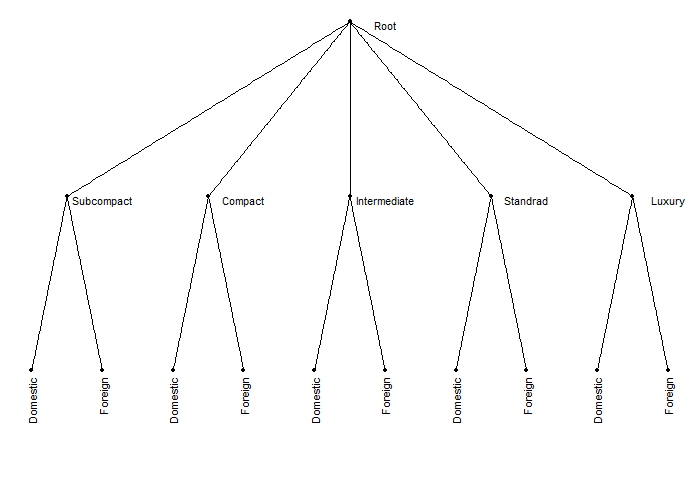
\includegraphics[width = 12cm,height = 8cm]{emp_plot.png}
        \caption{Nested Logit Structure for European Car Sales: Two-level Decision Tree}
        \label{fig: Emp_Decision Tree}
    \end{figure}

    \newpage
    
    The utility model is assumed to follow the unit demand specification which implies the prices enter the model linearly. The market share of a product $j$, the market share of the product in its subgroup $h$ of group $g$, and the market share of the subgroup $h$ in group $g$ are calculated based on the method as described by Björnerstedt and Verboven (2016) in section 5.3.   


    \begin{equation*}
        \qquad \mathbf{s_{j} = \dfrac{q_{j}}{I}, \quad 
        s_{j|hg} = \dfrac{q_{j}}{\sum_{j \in H_{hg}} q_{j}}, \quad 
        s_{h|g} = \dfrac{\sum_{j \in H_{hg}} q_{j}}{\sum_{h = 1}^{H_{hg}}\sum_{j \in H_{hg}} q_{j}}, \quad 
        s_{0} = 1 - \dfrac{\sum_{j = 1}^{J} q_{j}}{I}} 
    \end{equation*}

    While $q_{j}$ the quantity of each type of car sold is available, the potential market size $I$ is defined through a proxy for the number of households, namely, the total population divided by $4$. These values are thereby used to calculate the market shares of the products.\\

    The nested logit model can now be estimated using linear regression with instrumental variables to account for the endogeneity of the price variable. Firstly, the vector product characteristics, $x_{jt}$ are used as instruments. The other instrument used in the estimation process can be derived from the exogenous characteristics of competing products which act as a proxy for the intensity of competition firms face. This is the sum of the product characteristics of products sharing the same cluster (that is market segment and foreign/domestic status) \cite{Goldberge&Verboven2001}. Therefore, the estimation model is as follows

    \begin{equation*}
        \qquad \mathbf{M\_ls = \beta_{1} \alpha price + \sigma_{1} M\_lsjh + \sigma_{2} M\_lshg + \beta_{2} horsepower + \beta_{3} fuel + \beta_{4} width + \beta_{5} height + \beta_{7} log\_pop}
    \end{equation*}
    \begin{equation*}
        \qquad \mathbf{x_{jt} = (horsepower, fuel, width, height)}
    \end{equation*}
    \begin{equation*}
        \qquad \mathbf{instr = horsepower+ fuel + width + height }
    \end{equation*}

    $M\_ls$ is the dependent variable $ln(s_{j}/s_{0}$, $M\_lsjh$ is the log of the product's market share in the selected subgroup $ln(s_{j|hg})$, and $M\_lshg$ is the log of the market share of the selected subgroup $ln(s_{h|g})$. $horsepower$, $fuel$, $width$, $height$ and $weight$ are the product characteristics $x_{jt}$ and $log_pop$ is the logarithmic expression of the population variable. $z_{jt}$ represents the instruments included in the estimation to account for the price endogeneity and $instr$ is the sum of the product characteristics.\\

    \newpage
    The parameters of interest are the price parameter, $\alpha$ and the nesting parameters, $\sigma_{1}$ and $\sigma_{2}$. The estimated values of the parameters are $\alpha = -0.038$, $\sigma_{1} = 0.907$ and $\sigma_{2} = 0.739$. These estimates satisfy the conditions of random utility maximization and indicate a high degree of correlation among the product alternatives within each nest. The first-stage test to check the validity of the instruments also gives significant results, an F-statistic of $130.023$.\\
    
    \begin{figure}[htb]
        \centering
        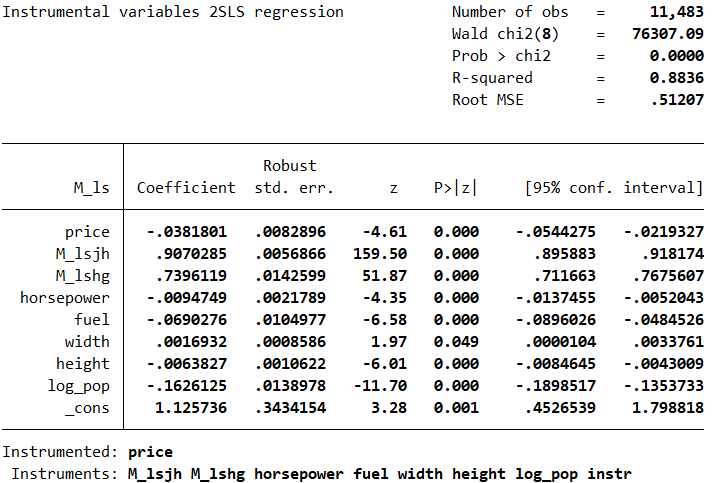
\includegraphics[width = 12cm,height = 8cm]{ivreg.PNG}
        \caption{Parameter Estimates for Nested Logit Model}
        \label{fig:Estimates}
    \end{figure}

    Before simulating a merger between the firms, it is necessary to evaluate the premerger market conditions. For this discussion, it is assumed that the firms' equilibrium behavior is defined by multiproduct Bertrand competition. The elasticity and firms' prices and marginal costs in the year 1990 for France have been discussed hereby. The cross-price elasticity values reveal distinct patterns in consumer preferences: products within the same subgroup exhibit a high cross-price elasticity of $0.643$, indicating that consumers view them as close substitutes and are highly likely to switch between them in response to price changes. In contrast, the elasticity between products from different subgroups is moderate at $0.129$, showing some degree of substitutability but less pronounced. Products from entirely different groups have an extremely low cross-price elasticity of $0.001$, reflecting minimal substitution and suggesting that consumers perceive these products as distinct and unrelated. Overall, these elasticity patterns highlight that consumer preferences are strongly aligned with the location where the cars are manufactured and the segment they belong to. The cross-price elasticities highlight The Lerner index denotes the percentage markup over marginal cost. It varies between $12\%$ and $35\%$ with the higher markup being associated with firms with lower-priced car models. The premerger market details for France for the year 1990 can be found below in Table 4 and Fig 8 in the Appendix.\\

    \begin{table}[h]
        \caption{France: Own- and Cross-Price Elasticities:  Unweighted Market Averages}
        \centering
        \begin{tabular}{ccccc}\\
            \hline
            Variable & Mean & SD & Min & Max\\ 
            \hline
            Own-Price Elasticity           & $-6.266$ & $2.989$ & $-18.461$ & $-2.660$\\
            Cross: same subgroup           & $0.643$  & $0.845$ & $0.004$ & $3.094$\\
            Cross: different subgroup      & $ 0.129$  & $0.215$ & $0.001$ & $0.902$\\
            Cross: different group         & $0.001$  & $0.002$ & $0.000$ & $0.006$\\
            \hline
            Observations : $78$\\
            \hline\\
        \end{tabular}
        \label{tab: France: Elasticity} 
    \end{table}


    Finally, a horizontal merger between two domestic firms in France is simulated to comprehend the effect of the anti-competitive practice on market conditions for the year 1990. In France, it is assumed that a merger will take place between PSA and Renault, where PSA will sell the brands Peugeot and Citröen. Further, the merger participants have been assumed to not have any marginal cost savings. Horizontal mergers are often scrutinized due to their tendency to accumulate market power and influence product prices. The results show the average pre and post-merger prices (Figure 8 in the Appendix) and the percentage price change for the firms operating in France. The merger predicts that on average the prices of PSA will increase by $43.1\%$ and of Renault by $52.3\%$. Figure 4 below visualizes the percentage change in prices.\\ 

    \begin{figure}[htb]
        \centering
        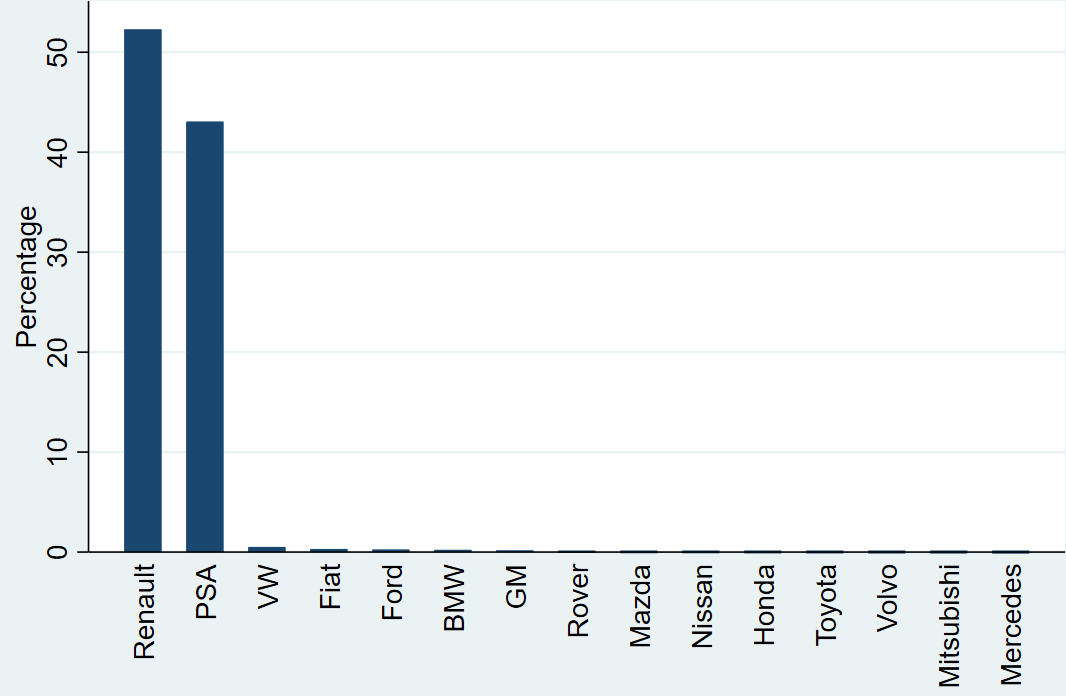
\includegraphics[width = 12cm,height = 8cm]{price_change_france.png}
        \caption{Average Percentage Price Increase Per Firm in France}
        \label{fig: Price Increase}
    \end{figure}
    
    The post-merger results also convey information on the market share of the 4 largest firms (C4) which increases to $80.65\%$. Herfindahl-Hirschman Index (HHI) is used to assess the level of market concentration before and after the merger. The index increases from $2209$ to $2346$. Since the simulation is based on a market with differentiated products, the index reports a concentrated market even without the merger. Post-merger, the market is seen to become more uncompetitive. This result is also corroborated by the change in market welfare. The consumer surplus falls by about $6.57$ billion Euro which is partly compensated by the rise in producer surplus of around $3.69$ billion Euro (Figure 9 in the Appendix).\\

   
    The competition authorities often undertake remedy measures like 'Divestiture' to mitigate the price effects of a merger and maintain competitiveness in the market. Under divestiture, the governing body allows the merger under the condition that the firm sells some of its products or brands. In the above example for France, the merger between PSA and Renault led to a significant increase in prices which consequently caused a huge consumer loss. Divestiture in this scenario would imply that the merger between the two firms would occur if PSA considers selling one of its brands to another firm. It is assumed that PSA sells its brand of Peugeot to the firm Ford. The merger results after incorporating divestiture differ from the previous results without any anticompetitive remedies as follows. In the new merger, the price effects are more dampened with no significant increase. Divestiture raises the average price by only $5\%$ for Renault and $2\%$ for Ford, which now includes Peugeot as well. On the other hand, the average price of cars sold by PSA falls by $4\%$. The impact of these price effects is also visible on market welfare, where the consumer surplus increases by $115,774$ Euro and the producer surplus falls by $24,089$ Euro.\\

    The nested logit model within the BLP framework plays a pivotal role in analyzing consumer choice and market dynamics. By leveraging the model's parameter estimates, researchers can calculate cross-elasticities, which provide insights into the correlation between products and the degree of substitution among them. These estimates are instrumental in assessing how market competition influences consumer welfare. For instance, the example provided demonstrates how the model can simulate firm mergers—an important market shock—and evaluate its effects on market competition through market share calculations and on overall welfare by assessing changes in consumer and producer surplus. This comprehensive approach highlights the model's relevance for both academic research and practical market analysis.\\
    
    \begin{figure}[htb]
        \centering
        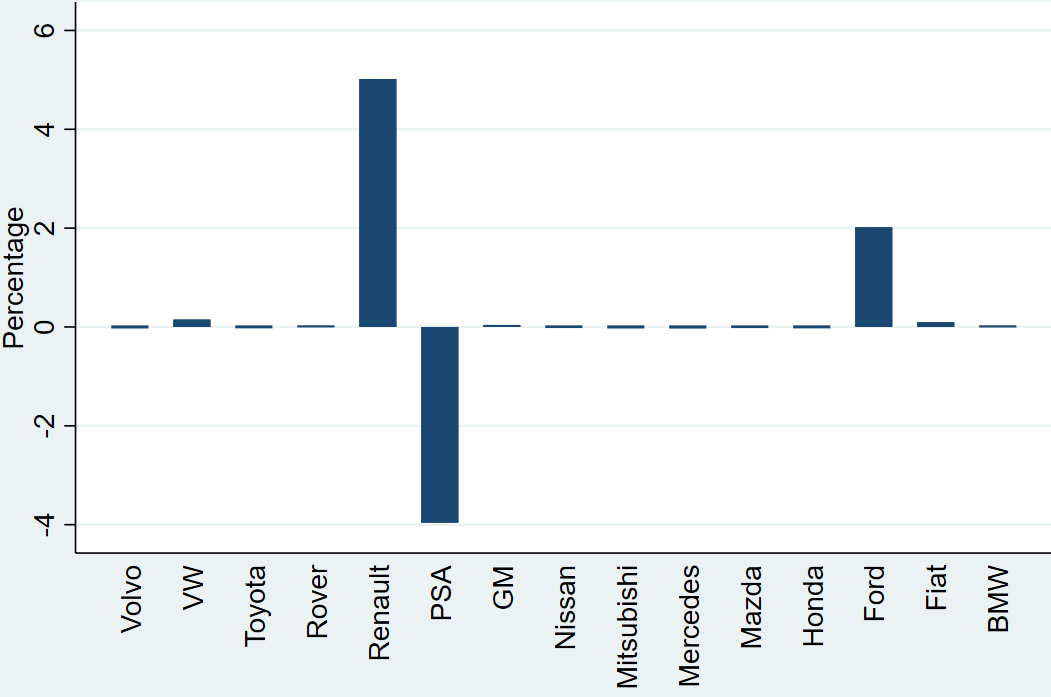
\includegraphics[width = 12cm,height = 8cm]{price_change_france_divest.png}
        \caption{Average Percentage Price Increase Per Firm in France post Divestiture}
        \label{fig: Price Increase Divest}
    \end{figure}

    \begin{figure}[htb]
        \centering
        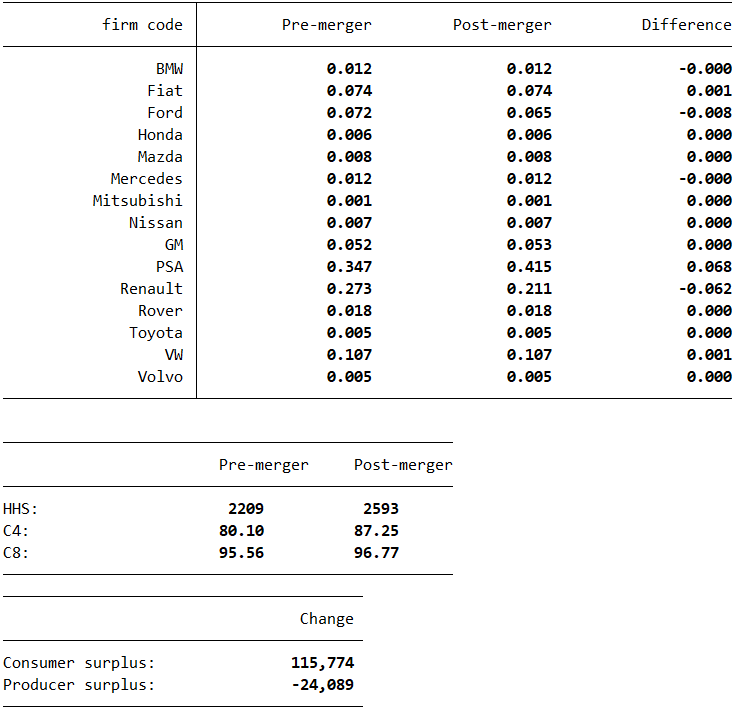
\includegraphics[width = 12cm,height = 8cm]{share_change_france_divest.png}
        \caption{Average Change in Market Shares and Market Welfare in France post Divestiture}
        \label{fig: Avg Change Divest}
    \end{figure}


\clearpage
\section{Conclusion}
\phantomsection\label{sec:Conclusion}

    Discrete choice models are commonly used to answer research questions where the dependent variable is categorical. These models are based on the assumption of 'Random Utility Maximization' (RUM) which states the choice maker's primary objective is to maximize his utility. The multinomial logit (MNL) and nested logit (NL) models are the two most commonly used discrete choice models due to their simplistic mathematical structures and ease of estimation. The assumption that the error terms in the models follow iid Type 1 Gumbel distribution, leads to a closed-form analytic solution for the choice probability. However, The difference between the two models arises through the property of 'Independence and Irrelevant Alternatives'. The IIA property implies that the relative odds of choosing between any two options should not change if a third option is added or removed, which can lead to unrealistic predictions in situations where adding or removing options significantly affects the relative attractiveness of the other choices. The nested logit model overcomes the challenge of the IIA property in the MNL by accounting for the substitution patterns of consumers between alternative products. These substitution patterns help the researcher to incorporate the complexity of decision-making processes to a greater extent than the MNL model. The BLP model is commonly used to estimate the demand parameters in a differentiated products market. The model estimates these parameters while considering the consumer heterogeneity and price endogeneity that is not fully explained by observed characteristics. However, this model tends to be computationally intensive and is also one of the motivations for applying the nested logit model under the BLP framework.\\
    
    Based on the simulation study, the Nested Logit (NL) model demonstrates clear advantages over the Multinomial Logit (MNL) model within the BLP framework. The empirical application also underscores the NL model's potential for analyzing market competition.\\ 
    
    In the simulation study, the nesting parameters under the NL model are correctly predicted in line with the principle of RUM as seen in Figure 7 in the Appendix. The results from the study corroborate the economic theory, primarily highlighting the flawed inference of the cross-elasticity estimates in the MNL model. It underscores the NL model's superior ability to handle endogeneity and capture complex substitution patterns among products. This implies that the segments capture the important role unobserved characteristics play in consumers' choice of alternatives. Even in terms of statistical performance, the MNL model is rejected in favor of the NL model. The NL model yields lower AIC and BIC values, indicating a better fit and more efficient use of data. Furthermore, the likelihood ratio test strongly supports the NL model's fit over the MNL model, reinforcing its robustness.\\
    
    The empirical application analyzes the use of the target model structure in interpreting the market outcomes. Using the market-level dataset on car sales and specifying the two-level nesting structure of the NL model, demand estimates were drawn. These estimates were thereby used to simulate firm mergers to understand the impact of change in market competition on the overall market welfare. A particularly relevant aspect of consumer heterogeneity
    was the cars domestic/foreign origin, which the NL model captured reasonably well. The difference in cross-price elasticity of alternatives belonging to the same and different subgroups within the same nest highlights that the origin of the car defines consumer preference as well. The merger also informs that the merger will entail high price effects if the merging firms sell close substitutes with respect to each other. Therefore, the price effects are more pronounced on domestic firms than the foreign firms in France. Divestiture as a remedy for monopoly behavior does curtail the huge price effects and ensures the limited impact of the merger on overall market efficiency. Thus, the two-level nested logit model can be a valuable tool for understanding the dynamics of market shocks such as firm mergers.\\

    The topic presents substantial opportunities for further application and research. Potential avenues include extending the model with alternative functional forms of demand, such as the random coefficients nested logit model and the cross-nested logit model. Additionally, employing constant expenditures utility specification could be investigated for enhanced accuracy of predictions. The logarithmic form of price in this indirect utility function may generate different results for elasticity and merger effects compared to unit demand.\\ 

\printbibliography

\clearpage
\pagenumbering{roman}
\setcounter{page}{1}

\section{Appendix}
\phantomsection\label{sec:Appendix}

    \begin{figure}[htb]
        \centering
        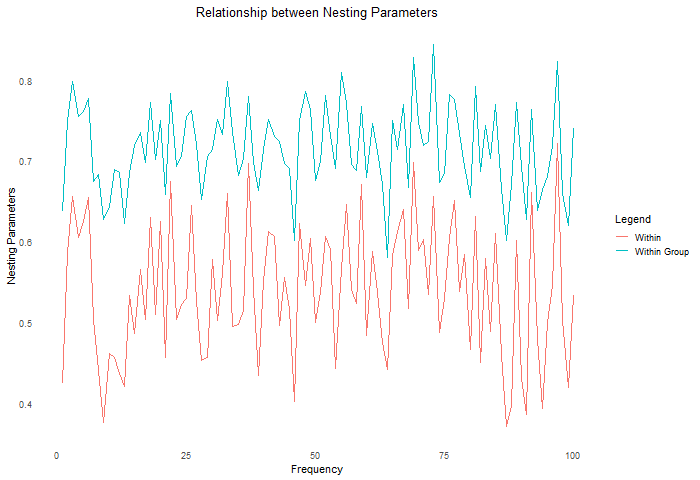
\includegraphics[width = 12cm,height = 8cm]{rum_plot.png}
        \caption{Nesting Parameters for random 100 datasets in the simulation study to corroborate the validity of the 'Random Utility Maximization' principles}
        \label{fig:RUM}
    \end{figure}

    \begin{figure}[htb]
        \centering
        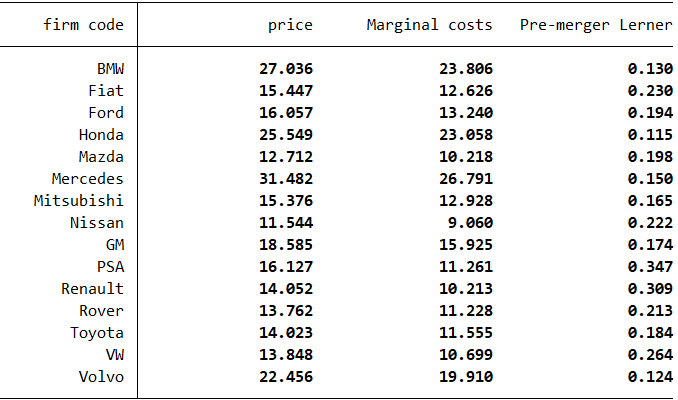
\includegraphics[width = 12cm,height = 8cm]{France_Pre_merger1990.png}
        \caption{Pre-Merger Market Conditions in France}
        \label{fig:France: Pre-Merger}
    \end{figure}

    \begin{figure}[htb]
        \centering
        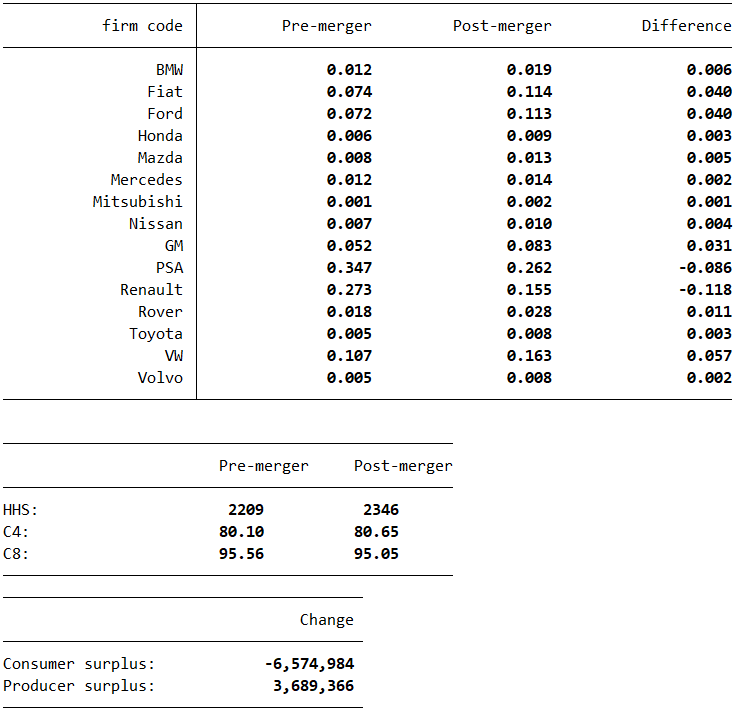
\includegraphics[width = 12cm,height = 8cm]{share_change_france.png}
        \caption{Average Change in Market Shares and Market Welfare in France}
        \label{fig: Avg Change}
    \end{figure}

\clearpage

\section{Statement of Authorship}
\phantomsection\label{sec:Statement}

"Ich versichere hiermit, dass ich die vorstehende Masterarbeit selbstständig verfasst und keine anderen als die angegebenen Quellen und Hilfsmittel benutzt habe, dass die vorgelegte Arbeit noch an keiner anderen Hochschule zur Prüfung vorgelegt wurde und dass sie weder ganz noch in Teilen bereits veröffentlicht wurde. Wörtliche Zitate und Stellen, die an- deren Werken dem Sinn nach entnommen sind, habe ich in jedem einzelnen Fall kenntlich gemacht."\\

"I hereby confirm that the work presented has been performed and interpreted solely by myself, except for where I explicitly identified the contrary. I assure that this work has not been presented in any other form for the fulfillment of any other degree or qualification. Ideas taken from other works in letter and in spirit are identified in every single case."\\

\vspace{2cm} % Adjust vertical space as needed
Date: \underline{\hspace{3cm}} \hfill Signature: \underline{\hspace{5cm}}

    
    
\end{document}